% Options for packages loaded elsewhere
\PassOptionsToPackage{unicode}{hyperref}
\PassOptionsToPackage{hyphens}{url}
%
\documentclass[
]{book}
\usepackage{amsmath,amssymb}
\usepackage{iftex}
\ifPDFTeX
  \usepackage[T1]{fontenc}
  \usepackage[utf8]{inputenc}
  \usepackage{textcomp} % provide euro and other symbols
\else % if luatex or xetex
  \usepackage{unicode-math} % this also loads fontspec
  \defaultfontfeatures{Scale=MatchLowercase}
  \defaultfontfeatures[\rmfamily]{Ligatures=TeX,Scale=1}
\fi
\usepackage{lmodern}
\ifPDFTeX\else
  % xetex/luatex font selection
\fi
% Use upquote if available, for straight quotes in verbatim environments
\IfFileExists{upquote.sty}{\usepackage{upquote}}{}
\IfFileExists{microtype.sty}{% use microtype if available
  \usepackage[]{microtype}
  \UseMicrotypeSet[protrusion]{basicmath} % disable protrusion for tt fonts
}{}
\makeatletter
\@ifundefined{KOMAClassName}{% if non-KOMA class
  \IfFileExists{parskip.sty}{%
    \usepackage{parskip}
  }{% else
    \setlength{\parindent}{0pt}
    \setlength{\parskip}{6pt plus 2pt minus 1pt}}
}{% if KOMA class
  \KOMAoptions{parskip=half}}
\makeatother
\usepackage{xcolor}
\usepackage{color}
\usepackage{fancyvrb}
\newcommand{\VerbBar}{|}
\newcommand{\VERB}{\Verb[commandchars=\\\{\}]}
\DefineVerbatimEnvironment{Highlighting}{Verbatim}{commandchars=\\\{\}}
% Add ',fontsize=\small' for more characters per line
\usepackage{framed}
\definecolor{shadecolor}{RGB}{248,248,248}
\newenvironment{Shaded}{\begin{snugshade}}{\end{snugshade}}
\newcommand{\AlertTok}[1]{\textcolor[rgb]{0.94,0.16,0.16}{#1}}
\newcommand{\AnnotationTok}[1]{\textcolor[rgb]{0.56,0.35,0.01}{\textbf{\textit{#1}}}}
\newcommand{\AttributeTok}[1]{\textcolor[rgb]{0.13,0.29,0.53}{#1}}
\newcommand{\BaseNTok}[1]{\textcolor[rgb]{0.00,0.00,0.81}{#1}}
\newcommand{\BuiltInTok}[1]{#1}
\newcommand{\CharTok}[1]{\textcolor[rgb]{0.31,0.60,0.02}{#1}}
\newcommand{\CommentTok}[1]{\textcolor[rgb]{0.56,0.35,0.01}{\textit{#1}}}
\newcommand{\CommentVarTok}[1]{\textcolor[rgb]{0.56,0.35,0.01}{\textbf{\textit{#1}}}}
\newcommand{\ConstantTok}[1]{\textcolor[rgb]{0.56,0.35,0.01}{#1}}
\newcommand{\ControlFlowTok}[1]{\textcolor[rgb]{0.13,0.29,0.53}{\textbf{#1}}}
\newcommand{\DataTypeTok}[1]{\textcolor[rgb]{0.13,0.29,0.53}{#1}}
\newcommand{\DecValTok}[1]{\textcolor[rgb]{0.00,0.00,0.81}{#1}}
\newcommand{\DocumentationTok}[1]{\textcolor[rgb]{0.56,0.35,0.01}{\textbf{\textit{#1}}}}
\newcommand{\ErrorTok}[1]{\textcolor[rgb]{0.64,0.00,0.00}{\textbf{#1}}}
\newcommand{\ExtensionTok}[1]{#1}
\newcommand{\FloatTok}[1]{\textcolor[rgb]{0.00,0.00,0.81}{#1}}
\newcommand{\FunctionTok}[1]{\textcolor[rgb]{0.13,0.29,0.53}{\textbf{#1}}}
\newcommand{\ImportTok}[1]{#1}
\newcommand{\InformationTok}[1]{\textcolor[rgb]{0.56,0.35,0.01}{\textbf{\textit{#1}}}}
\newcommand{\KeywordTok}[1]{\textcolor[rgb]{0.13,0.29,0.53}{\textbf{#1}}}
\newcommand{\NormalTok}[1]{#1}
\newcommand{\OperatorTok}[1]{\textcolor[rgb]{0.81,0.36,0.00}{\textbf{#1}}}
\newcommand{\OtherTok}[1]{\textcolor[rgb]{0.56,0.35,0.01}{#1}}
\newcommand{\PreprocessorTok}[1]{\textcolor[rgb]{0.56,0.35,0.01}{\textit{#1}}}
\newcommand{\RegionMarkerTok}[1]{#1}
\newcommand{\SpecialCharTok}[1]{\textcolor[rgb]{0.81,0.36,0.00}{\textbf{#1}}}
\newcommand{\SpecialStringTok}[1]{\textcolor[rgb]{0.31,0.60,0.02}{#1}}
\newcommand{\StringTok}[1]{\textcolor[rgb]{0.31,0.60,0.02}{#1}}
\newcommand{\VariableTok}[1]{\textcolor[rgb]{0.00,0.00,0.00}{#1}}
\newcommand{\VerbatimStringTok}[1]{\textcolor[rgb]{0.31,0.60,0.02}{#1}}
\newcommand{\WarningTok}[1]{\textcolor[rgb]{0.56,0.35,0.01}{\textbf{\textit{#1}}}}
\usepackage{longtable,booktabs,array}
\usepackage{calc} % for calculating minipage widths
% Correct order of tables after \paragraph or \subparagraph
\usepackage{etoolbox}
\makeatletter
\patchcmd\longtable{\par}{\if@noskipsec\mbox{}\fi\par}{}{}
\makeatother
% Allow footnotes in longtable head/foot
\IfFileExists{footnotehyper.sty}{\usepackage{footnotehyper}}{\usepackage{footnote}}
\makesavenoteenv{longtable}
\usepackage{graphicx}
\makeatletter
\def\maxwidth{\ifdim\Gin@nat@width>\linewidth\linewidth\else\Gin@nat@width\fi}
\def\maxheight{\ifdim\Gin@nat@height>\textheight\textheight\else\Gin@nat@height\fi}
\makeatother
% Scale images if necessary, so that they will not overflow the page
% margins by default, and it is still possible to overwrite the defaults
% using explicit options in \includegraphics[width, height, ...]{}
\setkeys{Gin}{width=\maxwidth,height=\maxheight,keepaspectratio}
% Set default figure placement to htbp
\makeatletter
\def\fps@figure{htbp}
\makeatother
\setlength{\emergencystretch}{3em} % prevent overfull lines
\providecommand{\tightlist}{%
  \setlength{\itemsep}{0pt}\setlength{\parskip}{0pt}}
\setcounter{secnumdepth}{5}
\usepackage{booktabs}
\ifLuaTeX
  \usepackage{selnolig}  % disable illegal ligatures
\fi
\usepackage[]{natbib}
\bibliographystyle{plainnat}
\IfFileExists{bookmark.sty}{\usepackage{bookmark}}{\usepackage{hyperref}}
\IfFileExists{xurl.sty}{\usepackage{xurl}}{} % add URL line breaks if available
\urlstyle{same}
\hypersetup{
  pdftitle={Aprendendo R},
  pdfauthor={Magno TF Severino},
  hidelinks,
  pdfcreator={LaTeX via pandoc}}

\title{Aprendendo R}
\author{Magno TF Severino}
\date{2023-12-23}

\begin{document}
\maketitle

{
\setcounter{tocdepth}{1}
\tableofcontents
}
\chapter*{Introdução}\label{introduuxe7uxe3o}
\addcontentsline{toc}{chapter}{Introdução}

Este livro compila tutoriais da linguagem \texttt{R} que usei em diversas aulas que dei ao longo dos últimos anos e foi escrito baseado em Cotton (2013)

\chapter{\texorpdfstring{Básicos da linguagem \texttt{R}}{Básicos da linguagem R}}\label{buxe1sicos-da-linguagem-r}

\begin{quote}
O conteúdo apresentado aqui foi usado na primeira aula prática do curso de ``Aprendizagem Estatística com Aplicações em R''.
\end{quote}

Para instalação,

\begin{itemize}
\item
  faça o download do R em \url{http://www.r-project.org};
\item
  sugestão: utilizar a IDE \href{http://www.rstudio.org}{R Studio}.
\end{itemize}

É muito importante saber como obter ajuda no R.
Sempre que estiver em dúvidas quanto as características de alguma função, consule a aba \emph{help} do RStudio.

\begin{Shaded}
\begin{Highlighting}[]
\NormalTok{?mean }\CommentTok{\#abre a página de ajuda da função \textquotesingle{}mean\textquotesingle{}}
\NormalTok{??plot }\CommentTok{\#procura por tópicos contendo a palavra \textquotesingle{}plot\textquotesingle{}}
\end{Highlighting}
\end{Shaded}

\section{\texorpdfstring{Usando o \texttt{R} como uma calculadora}{Usando o R como uma calculadora}}\label{usando-o-r-como-uma-calculadora}

O operador + realiza a adição entre dois elementos.

\begin{Shaded}
\begin{Highlighting}[]
\DecValTok{1} \SpecialCharTok{+} \DecValTok{2}
\end{Highlighting}
\end{Shaded}

\begin{verbatim}
## [1] 3
\end{verbatim}

Um vetor é um conjunto ordenado de valores.
O operador : cria uma sequência a partir de um número até outro.
A função c concatena valores, criando um vetor.

\begin{Shaded}
\begin{Highlighting}[]
\DecValTok{1}\SpecialCharTok{:}\DecValTok{5}
\end{Highlighting}
\end{Shaded}

\begin{verbatim}
## [1] 1 2 3 4 5
\end{verbatim}

\begin{Shaded}
\begin{Highlighting}[]
\FunctionTok{c}\NormalTok{(}\DecValTok{1}\NormalTok{, }\DecValTok{2}\NormalTok{, }\DecValTok{3}\NormalTok{, }\DecValTok{4}\NormalTok{, }\DecValTok{5}\NormalTok{)}
\end{Highlighting}
\end{Shaded}

\begin{verbatim}
## [1] 1 2 3 4 5
\end{verbatim}

Além de adicionar dois números, o operador + pode ser usado para adicionar dois vetores.

\begin{Shaded}
\begin{Highlighting}[]
\DecValTok{1}\SpecialCharTok{:}\DecValTok{5} \SpecialCharTok{+} \DecValTok{6}\SpecialCharTok{:}\DecValTok{10}
\end{Highlighting}
\end{Shaded}

\begin{verbatim}
## [1]  7  9 11 13 15
\end{verbatim}

\begin{Shaded}
\begin{Highlighting}[]
\FunctionTok{c}\NormalTok{(}\DecValTok{1}\NormalTok{, }\DecValTok{2}\NormalTok{, }\DecValTok{3}\NormalTok{, }\DecValTok{4}\NormalTok{, }\DecValTok{5}\NormalTok{) }\SpecialCharTok{+} \FunctionTok{c}\NormalTok{(}\DecValTok{6}\NormalTok{, }\DecValTok{7}\NormalTok{, }\DecValTok{8}\NormalTok{, }\DecValTok{9}\NormalTok{, }\DecValTok{10}\NormalTok{)}
\end{Highlighting}
\end{Shaded}

\begin{verbatim}
## [1]  7  9 11 13 15
\end{verbatim}

\begin{Shaded}
\begin{Highlighting}[]
\DecValTok{1}\SpecialCharTok{:}\DecValTok{5} \SpecialCharTok{+} \FunctionTok{c}\NormalTok{(}\DecValTok{6}\NormalTok{, }\DecValTok{7}\NormalTok{, }\DecValTok{8}\NormalTok{, }\DecValTok{9}\NormalTok{, }\DecValTok{10}\NormalTok{)}
\end{Highlighting}
\end{Shaded}

\begin{verbatim}
## [1]  7  9 11 13 15
\end{verbatim}

Os próximos exemplos mostram subtração, multiplicação, exponenciação e divisão.

\begin{Shaded}
\begin{Highlighting}[]
\FunctionTok{c}\NormalTok{(}\DecValTok{2}\NormalTok{, }\DecValTok{3}\NormalTok{, }\DecValTok{5}\NormalTok{, }\DecValTok{7}\NormalTok{, }\DecValTok{11}\NormalTok{, }\DecValTok{13}\NormalTok{) }\SpecialCharTok{{-}} \DecValTok{2}       \CommentTok{\#subtração}
\end{Highlighting}
\end{Shaded}

\begin{verbatim}
## [1]  0  1  3  5  9 11
\end{verbatim}

\begin{Shaded}
\begin{Highlighting}[]
\SpecialCharTok{{-}}\DecValTok{2}\SpecialCharTok{:}\DecValTok{2} \SpecialCharTok{*} \SpecialCharTok{{-}}\DecValTok{2}\SpecialCharTok{:}\DecValTok{2}                     \CommentTok{\#multiplicação}
\end{Highlighting}
\end{Shaded}

\begin{verbatim}
## [1] 4 1 0 1 4
\end{verbatim}

\begin{Shaded}
\begin{Highlighting}[]
\NormalTok{(}\DecValTok{1}\SpecialCharTok{:}\DecValTok{10}\NormalTok{) }\SpecialCharTok{\^{}} \DecValTok{2}                        \CommentTok{\#exponenciação}
\end{Highlighting}
\end{Shaded}

\begin{verbatim}
##  [1]   1   4   9  16  25  36  49  64  81 100
\end{verbatim}

\begin{Shaded}
\begin{Highlighting}[]
\DecValTok{1}\SpecialCharTok{:}\DecValTok{10} \SpecialCharTok{/} \DecValTok{3}                        \CommentTok{\#divisão}
\end{Highlighting}
\end{Shaded}

\begin{verbatim}
##  [1] 0.3333333 0.6666667 1.0000000 1.3333333 1.6666667 2.0000000 2.3333333
##  [8] 2.6666667 3.0000000 3.3333333
\end{verbatim}

\section{Atribuindo variáveis}\label{atribuindo-variuxe1veis}

Fazer cálculos com o R é bem simples e útil.
A maior parte das vezes queremos armazenar os resultados para uso posterior.
Assim, podemos atribuir valor à uma variável, através do operador \textless-.

\begin{Shaded}
\begin{Highlighting}[]
\NormalTok{a }\OtherTok{\textless{}{-}} \DecValTok{1}

\NormalTok{b }\OtherTok{\textless{}{-}} \DecValTok{5} \SpecialCharTok{*} \DecValTok{3}

\NormalTok{x }\OtherTok{\textless{}{-}} \DecValTok{1}\SpecialCharTok{:}\DecValTok{5}

\NormalTok{y }\OtherTok{\textless{}{-}} \DecValTok{6}\SpecialCharTok{:}\DecValTok{10}
\end{Highlighting}
\end{Shaded}

Agora, podemos reutilizar esses valores para fazer outros cálculos.

\begin{Shaded}
\begin{Highlighting}[]
\NormalTok{a }\SpecialCharTok{+} \DecValTok{2} \SpecialCharTok{*}\NormalTok{ b}
\end{Highlighting}
\end{Shaded}

\begin{verbatim}
## [1] 31
\end{verbatim}

\begin{Shaded}
\begin{Highlighting}[]
\NormalTok{x }\SpecialCharTok{+} \DecValTok{2} \SpecialCharTok{*}\NormalTok{ y }\SpecialCharTok{{-}} \DecValTok{3}
\end{Highlighting}
\end{Shaded}

\begin{verbatim}
## [1] 10 13 16 19 22
\end{verbatim}

Observe que não temos que dizer ao R qual o tipo da variável, se era um número (as variáveis a e a) ou vetor (x e y).

\section{Números especias}\label{nuxfameros-especias}

Para facilitar operações aritméticas, R suporta quatro valores especiais de números: Inf, -Inf, NaN e NA.
Os dois primeiros representam infinito positivo e negativo.
NaN é um acrônimo inglês para ``not a number'', ou seja, não é um número.
Ele aparece quando um cálculo não faz sentido, ou não está definido.
NA significa ``not available'', ou seja, não disponível, e representa um valor faltante.

\begin{Shaded}
\begin{Highlighting}[]
\FunctionTok{c}\NormalTok{(}\ConstantTok{Inf} \SpecialCharTok{+} \DecValTok{1}\NormalTok{, }\ConstantTok{Inf} \SpecialCharTok{{-}} \DecValTok{1}\NormalTok{, }\ConstantTok{Inf} \SpecialCharTok{{-}} \ConstantTok{Inf}\NormalTok{, }\ConstantTok{NA} \SpecialCharTok{+} \DecValTok{1}\NormalTok{)}
\end{Highlighting}
\end{Shaded}

\begin{verbatim}
## [1] Inf Inf NaN  NA
\end{verbatim}

\begin{Shaded}
\begin{Highlighting}[]
\FunctionTok{c}\NormalTok{(}\DecValTok{0} \SpecialCharTok{/} \DecValTok{0}\NormalTok{, }\ConstantTok{Inf} \SpecialCharTok{/} \ConstantTok{Inf}\NormalTok{, }\DecValTok{1} \SpecialCharTok{/} \ConstantTok{Inf}\NormalTok{)}
\end{Highlighting}
\end{Shaded}

\begin{verbatim}
## [1] NaN NaN   0
\end{verbatim}

\section{Vetores, Matrizes e Dataframes}\label{vetores-matrizes-e-dataframes}

Previamente, vimos alguns tipos de vetores para valores lógicos, caracteres e números.
Nessa seção, utilizaremos técnicas de manipulação de vetores e introduziremos o caso multidimensional: matrizes e dataframes.

Abaixo relembramos as operações que já foram feitas com vetores

\begin{Shaded}
\begin{Highlighting}[]
\DecValTok{10}\SpecialCharTok{:}\DecValTok{5}                    \CommentTok{\#sequência de números de 10 até 5}
\end{Highlighting}
\end{Shaded}

\begin{verbatim}
## [1] 10  9  8  7  6  5
\end{verbatim}

\begin{Shaded}
\begin{Highlighting}[]
\FunctionTok{c}\NormalTok{(}\DecValTok{1}\NormalTok{, }\DecValTok{2}\SpecialCharTok{:}\DecValTok{5}\NormalTok{, }\FunctionTok{c}\NormalTok{(}\DecValTok{6}\NormalTok{, }\DecValTok{7}\NormalTok{), }\DecValTok{8}\NormalTok{)   }\CommentTok{\#valores concatenados em um único vetor}
\end{Highlighting}
\end{Shaded}

\begin{verbatim}
## [1] 1 2 3 4 5 6 7 8
\end{verbatim}

\subsection{Vetores}\label{vetores}

Existem funções para criar vetores de um tipo e com tamanho específicos.
Todos os elementos deste vetor terá valor zero, FALSE, um caracter vazio, ou o equivalente à \emph{nada/vazio} para aquele tipo.
Veja abaixo duas maneiras de definir um vetor.

\begin{Shaded}
\begin{Highlighting}[]
\FunctionTok{vector}\NormalTok{(}\StringTok{"numeric"}\NormalTok{, }\DecValTok{5}\NormalTok{) }\CommentTok{\#cria um vetor numérico de 5 elementos}
\end{Highlighting}
\end{Shaded}

\begin{verbatim}
## [1] 0 0 0 0 0
\end{verbatim}

\begin{Shaded}
\begin{Highlighting}[]
\FunctionTok{numeric}\NormalTok{(}\DecValTok{5}\NormalTok{) }\CommentTok{\#equivalente ao comando acima}
\end{Highlighting}
\end{Shaded}

\begin{verbatim}
## [1] 0 0 0 0 0
\end{verbatim}

\begin{Shaded}
\begin{Highlighting}[]
\FunctionTok{vector}\NormalTok{(}\StringTok{"logical"}\NormalTok{, }\DecValTok{5}\NormalTok{) }\CommentTok{\#cria um vetor lógico de 5 elementos}
\end{Highlighting}
\end{Shaded}

\begin{verbatim}
## [1] FALSE FALSE FALSE FALSE FALSE
\end{verbatim}

\begin{Shaded}
\begin{Highlighting}[]
\FunctionTok{logical}\NormalTok{(}\DecValTok{5}\NormalTok{) }\CommentTok{\#equivalente ao comando acima}
\end{Highlighting}
\end{Shaded}

\begin{verbatim}
## [1] FALSE FALSE FALSE FALSE FALSE
\end{verbatim}

\begin{Shaded}
\begin{Highlighting}[]
\FunctionTok{vector}\NormalTok{(}\StringTok{"character"}\NormalTok{, }\DecValTok{5}\NormalTok{) }\CommentTok{\#cria um vetor de caracteres de 5 elementos}
\end{Highlighting}
\end{Shaded}

\begin{verbatim}
## [1] "" "" "" "" ""
\end{verbatim}

\begin{Shaded}
\begin{Highlighting}[]
\FunctionTok{character}\NormalTok{(}\DecValTok{5}\NormalTok{) }\CommentTok{\#equivalente ao comando acima}
\end{Highlighting}
\end{Shaded}

\begin{verbatim}
## [1] "" "" "" "" ""
\end{verbatim}

\subsubsection{Sequências}\label{S:sequencia}

Podemos criar sequências mais gerais que aquelas criadas com o operador :.
A função seq te permite criar sequências em diferentes maneiras
Veja abaixo.

\begin{Shaded}
\begin{Highlighting}[]
\FunctionTok{seq}\NormalTok{(}\DecValTok{3}\NormalTok{, }\DecValTok{12}\NormalTok{) }\CommentTok{\#equivalente à 3:12}
\end{Highlighting}
\end{Shaded}

\begin{verbatim}
##  [1]  3  4  5  6  7  8  9 10 11 12
\end{verbatim}

\begin{Shaded}
\begin{Highlighting}[]
\FunctionTok{seq}\NormalTok{(}\DecValTok{3}\NormalTok{, }\DecValTok{12}\NormalTok{, }\DecValTok{2}\NormalTok{) }\CommentTok{\#o terceiro argumento indica a distância entre os elementos na lista.}
\end{Highlighting}
\end{Shaded}

\begin{verbatim}
## [1]  3  5  7  9 11
\end{verbatim}

\begin{Shaded}
\begin{Highlighting}[]
\FunctionTok{seq}\NormalTok{(}\FloatTok{0.1}\NormalTok{, }\FloatTok{0.01}\NormalTok{, }\SpecialCharTok{{-}}\FloatTok{0.01}\NormalTok{)}
\end{Highlighting}
\end{Shaded}

\begin{verbatim}
##  [1] 0.10 0.09 0.08 0.07 0.06 0.05 0.04 0.03 0.02 0.01
\end{verbatim}

\subsubsection{Tamanhos}\label{tamanhos}

Todo vetor tem um tamanho, um número não negativo que representa a quantidade de elementos que o vetor contém.
A função length retorna o tamanho de um dado vetor.

\begin{Shaded}
\begin{Highlighting}[]
\FunctionTok{length}\NormalTok{(}\DecValTok{1}\SpecialCharTok{:}\DecValTok{5}\NormalTok{) }
\end{Highlighting}
\end{Shaded}

\begin{verbatim}
## [1] 5
\end{verbatim}

\begin{Shaded}
\begin{Highlighting}[]
\NormalTok{frase }\OtherTok{\textless{}{-}} \FunctionTok{c}\NormalTok{(}\StringTok{"Observe"}\NormalTok{, }\StringTok{"o"}\NormalTok{, }\StringTok{"resultado"}\NormalTok{, }\StringTok{"dos"}\NormalTok{, }\StringTok{"comandos"}\NormalTok{, }\StringTok{"abaixo"}\NormalTok{)}

\FunctionTok{length}\NormalTok{(frase)}
\end{Highlighting}
\end{Shaded}

\begin{verbatim}
## [1] 6
\end{verbatim}

\begin{Shaded}
\begin{Highlighting}[]
\FunctionTok{nchar}\NormalTok{(frase)}
\end{Highlighting}
\end{Shaded}

\begin{verbatim}
## [1] 7 1 9 3 8 6
\end{verbatim}

\subsubsection{Indexando vetores}\label{indexando-vetores}

A indexação é útil quando queremos acessar elementos específicos de um vetor.
Considere o vetor

\begin{Shaded}
\begin{Highlighting}[]
\NormalTok{x }\OtherTok{\textless{}{-}}\NormalTok{ (}\DecValTok{1}\SpecialCharTok{:}\DecValTok{5}\NormalTok{) }\SpecialCharTok{\^{}} \DecValTok{2}
\end{Highlighting}
\end{Shaded}

Abaixo, três métodos de indexar os mesmos valores do vetor x.

\begin{Shaded}
\begin{Highlighting}[]
\NormalTok{x[}\FunctionTok{c}\NormalTok{(}\DecValTok{1}\NormalTok{, }\DecValTok{3}\NormalTok{, }\DecValTok{5}\NormalTok{)]}

\NormalTok{x[}\FunctionTok{c}\NormalTok{(}\SpecialCharTok{{-}}\DecValTok{2}\NormalTok{, }\SpecialCharTok{{-}}\DecValTok{4}\NormalTok{)]}
\end{Highlighting}
\end{Shaded}

\begin{Shaded}
\begin{Highlighting}[]
\NormalTok{x[}\FunctionTok{c}\NormalTok{(}\ConstantTok{TRUE}\NormalTok{, }\ConstantTok{FALSE}\NormalTok{, }\ConstantTok{TRUE}\NormalTok{, }\ConstantTok{FALSE}\NormalTok{, }\ConstantTok{TRUE}\NormalTok{)]}
\end{Highlighting}
\end{Shaded}

\begin{verbatim}
## [1]  1  9 25
\end{verbatim}

Se nomearmos os elementos do vetor, o método abaixo obtém os mesmos valores de x.

\begin{Shaded}
\begin{Highlighting}[]
\FunctionTok{names}\NormalTok{(x) }\OtherTok{\textless{}{-}} \FunctionTok{c}\NormalTok{(}\StringTok{"one"}\NormalTok{, }\StringTok{"four"}\NormalTok{, }\StringTok{"nine"}\NormalTok{, }\StringTok{"sixteen"}\NormalTok{, }\StringTok{"twenty five"}\NormalTok{)}
\NormalTok{x[}\FunctionTok{c}\NormalTok{(}\StringTok{"one"}\NormalTok{, }\StringTok{"nine"}\NormalTok{, }\StringTok{"twenty five"}\NormalTok{)]}
\end{Highlighting}
\end{Shaded}

\begin{verbatim}
##         one        nine twenty five 
##           1           9          25
\end{verbatim}

Cuidado, acessar um elemento fora do tamanho do vetor não gera um erro no R, apenas NA.

\begin{Shaded}
\begin{Highlighting}[]
\NormalTok{x[}\DecValTok{6}\NormalTok{]}
\end{Highlighting}
\end{Shaded}

\begin{verbatim}
## <NA> 
##   NA
\end{verbatim}

\subsection{Matrizes}\label{matrizes}

Uma matriz é o equivalente à um vetor, porém em duas dimensões.
Abaixo, um exemplo de definição de uma matriz com 4 linhas e 3 colunas (total de 12 elementos).

\begin{Shaded}
\begin{Highlighting}[]
\NormalTok{?matrix}
\end{Highlighting}
\end{Shaded}

\begin{Shaded}
\begin{Highlighting}[]
\NormalTok{uma\_matriz }\OtherTok{\textless{}{-}} \FunctionTok{matrix}\NormalTok{(}
      \DecValTok{1}\SpecialCharTok{:}\DecValTok{12}\NormalTok{,}
      \AttributeTok{nrow =} \DecValTok{4}\NormalTok{, }\CommentTok{\#ncol = 3 gera o mesmo resultado. Verifique!}
      \AttributeTok{dimnames =} \FunctionTok{list}\NormalTok{(}
        \FunctionTok{c}\NormalTok{(}\StringTok{"L1"}\NormalTok{, }\StringTok{"L2"}\NormalTok{, }\StringTok{"L3"}\NormalTok{, }\StringTok{"L4"}\NormalTok{),}
        \FunctionTok{c}\NormalTok{(}\StringTok{"C1"}\NormalTok{, }\StringTok{"C2"}\NormalTok{, }\StringTok{"C3"}\NormalTok{)}
\NormalTok{      )}
\NormalTok{)}

\FunctionTok{class}\NormalTok{(uma\_matriz)}
\end{Highlighting}
\end{Shaded}

\begin{verbatim}
## [1] "matrix" "array"
\end{verbatim}

\begin{Shaded}
\begin{Highlighting}[]
\NormalTok{uma\_matriz}
\end{Highlighting}
\end{Shaded}

\begin{verbatim}
##    C1 C2 C3
## L1  1  5  9
## L2  2  6 10
## L3  3  7 11
## L4  4  8 12
\end{verbatim}

Por padrão, ao criar uma matrix, o vetor passado como primeiro argumento preenche a matrix por colunas.
Para preencher a matrix por linhas, basta especificar o argumento byrow=TRUE

A função dim retorna um vetor de inteiros com as dimensões da variável.

\begin{Shaded}
\begin{Highlighting}[]
\FunctionTok{dim}\NormalTok{(uma\_matriz)}
\end{Highlighting}
\end{Shaded}

\begin{verbatim}
## [1] 4 3
\end{verbatim}

\begin{Shaded}
\begin{Highlighting}[]
\FunctionTok{nrow}\NormalTok{(uma\_matriz) }\CommentTok{\#retorna o número de linhas da matrix}
\end{Highlighting}
\end{Shaded}

\begin{verbatim}
## [1] 4
\end{verbatim}

\begin{Shaded}
\begin{Highlighting}[]
\FunctionTok{ncol}\NormalTok{(uma\_matriz) }\CommentTok{\#retorna o número de colunas da matrix}
\end{Highlighting}
\end{Shaded}

\begin{verbatim}
## [1] 3
\end{verbatim}

\begin{Shaded}
\begin{Highlighting}[]
\FunctionTok{length}\NormalTok{(uma\_matriz) }\CommentTok{\#retorna o número de elementos da matrix}
\end{Highlighting}
\end{Shaded}

\begin{verbatim}
## [1] 12
\end{verbatim}

\subsubsection{Nomeando linhas, columas e dimensões}\label{nomeando-linhas-columas-e-dimensuxf5es}

Da mesma forma para vetores, podemos nomear (e obter os nomes de) linhas e colunas de matrizes.

\begin{Shaded}
\begin{Highlighting}[]
\FunctionTok{rownames}\NormalTok{(uma\_matriz)}
\end{Highlighting}
\end{Shaded}

\begin{verbatim}
## [1] "L1" "L2" "L3" "L4"
\end{verbatim}

\begin{Shaded}
\begin{Highlighting}[]
\FunctionTok{colnames}\NormalTok{(uma\_matriz)}
\end{Highlighting}
\end{Shaded}

\begin{verbatim}
## [1] "C1" "C2" "C3"
\end{verbatim}

\begin{Shaded}
\begin{Highlighting}[]
\FunctionTok{dimnames}\NormalTok{(uma\_matriz)}
\end{Highlighting}
\end{Shaded}

\begin{verbatim}
## [[1]]
## [1] "L1" "L2" "L3" "L4"
## 
## [[2]]
## [1] "C1" "C2" "C3"
\end{verbatim}

\subsubsection{Indexação}\label{indexauxe7uxe3o}

A indexação de matrizes funciona de maneira similar à de vetores, com a diferença que agora precisam ser especificadas mais de uma dimensão.

\begin{Shaded}
\begin{Highlighting}[]
\NormalTok{uma\_matriz[}\DecValTok{1}\NormalTok{, }\FunctionTok{c}\NormalTok{(}\StringTok{"C2"}\NormalTok{, }\StringTok{"C3"}\NormalTok{)] }\CommentTok{\#elementos na primeira linha, segunda e terceira colunas}
\end{Highlighting}
\end{Shaded}

\begin{verbatim}
## C2 C3 
##  5  9
\end{verbatim}

\begin{Shaded}
\begin{Highlighting}[]
\NormalTok{uma\_matriz[}\DecValTok{1}\NormalTok{, ] }\CommentTok{\#todos elementos da primeira linha}
\end{Highlighting}
\end{Shaded}

\begin{verbatim}
## C1 C2 C3 
##  1  5  9
\end{verbatim}

\begin{Shaded}
\begin{Highlighting}[]
\NormalTok{uma\_matriz[, }\FunctionTok{c}\NormalTok{(}\StringTok{"C2"}\NormalTok{, }\StringTok{"C3"}\NormalTok{)] }\CommentTok{\#todos elementos da segunda e terceira colunas}
\end{Highlighting}
\end{Shaded}

\begin{verbatim}
##    C2 C3
## L1  5  9
## L2  6 10
## L3  7 11
## L4  8 12
\end{verbatim}

\begin{Shaded}
\begin{Highlighting}[]
\NormalTok{uma\_matriz[, }\FunctionTok{c}\NormalTok{(}\DecValTok{2}\NormalTok{, }\DecValTok{3}\NormalTok{)] }\CommentTok{\#todos elementos da segunda e terceira colunas}
\end{Highlighting}
\end{Shaded}

\begin{verbatim}
##    C2 C3
## L1  5  9
## L2  6 10
## L3  7 11
## L4  8 12
\end{verbatim}

\subsubsection{Combinando matrizes}\label{combinando-matrizes}

Considere a seguinte matriz.

\begin{Shaded}
\begin{Highlighting}[]
\NormalTok{outra\_matriz }\OtherTok{\textless{}{-}} \FunctionTok{matrix}\NormalTok{(}
      \FunctionTok{seq}\NormalTok{(}\DecValTok{2}\NormalTok{, }\DecValTok{24}\NormalTok{, }\DecValTok{2}\NormalTok{),}
      \AttributeTok{nrow =} \DecValTok{4}\NormalTok{,}
      \AttributeTok{dimnames =} \FunctionTok{list}\NormalTok{(}
        \FunctionTok{c}\NormalTok{(}\StringTok{"L5"}\NormalTok{, }\StringTok{"L6"}\NormalTok{, }\StringTok{"L7"}\NormalTok{, }\StringTok{"L8"}\NormalTok{),}
        \FunctionTok{c}\NormalTok{(}\StringTok{"C5"}\NormalTok{, }\StringTok{"C6"}\NormalTok{, }\StringTok{"C7"}\NormalTok{)}
\NormalTok{      ))}
\end{Highlighting}
\end{Shaded}

A combinação de matrizes pode ser feita através das funções cbind e rbind, que combina matrizes por colunas e por linhas, respectivamentes.

\begin{Shaded}
\begin{Highlighting}[]
\FunctionTok{cbind}\NormalTok{(uma\_matriz, outra\_matriz)}
\end{Highlighting}
\end{Shaded}

\begin{verbatim}
##    C1 C2 C3 C5 C6 C7
## L1  1  5  9  2 10 18
## L2  2  6 10  4 12 20
## L3  3  7 11  6 14 22
## L4  4  8 12  8 16 24
\end{verbatim}

\begin{Shaded}
\begin{Highlighting}[]
\FunctionTok{rbind}\NormalTok{(uma\_matriz, outra\_matriz)}
\end{Highlighting}
\end{Shaded}

\begin{verbatim}
##    C1 C2 C3
## L1  1  5  9
## L2  2  6 10
## L3  3  7 11
## L4  4  8 12
## L5  2 10 18
## L6  4 12 20
## L7  6 14 22
## L8  8 16 24
\end{verbatim}

\subsubsection{Operações com matrizes}\label{operauxe7uxf5es-com-matrizes}

As operações básicas (+, -, *, /) funcionam de elemento a elemento em matrizes, da mesmo forma como em vetores:

\begin{Shaded}
\begin{Highlighting}[]
\NormalTok{uma\_matriz }\SpecialCharTok{+}\NormalTok{ outra\_matriz}
\end{Highlighting}
\end{Shaded}

\begin{verbatim}
##    C1 C2 C3
## L1  3 15 27
## L2  6 18 30
## L3  9 21 33
## L4 12 24 36
\end{verbatim}

\begin{Shaded}
\begin{Highlighting}[]
\NormalTok{uma\_matriz }\SpecialCharTok{*}\NormalTok{ outra\_matriz}
\end{Highlighting}
\end{Shaded}

\begin{verbatim}
##    C1  C2  C3
## L1  2  50 162
## L2  8  72 200
## L3 18  98 242
## L4 32 128 288
\end{verbatim}

Cuidado: as matrizes e vetores devem ter tamanhos compativeis!

\chapter{Controle de fluxo e repetição}\label{controle-de-fluxo-e-repetiuxe7uxe3o}

\begin{quote}
Este capítulo foi escrito baseado em Cotton (2013) e o conteúdo apresentado aqui foi usado como base para o minicurso ``R para não-programadores''.
\end{quote}

Por algum motivo particular, você pode querer executar ou não um determinado trecho do seu código.
Também, pode querer que um trecho seja executado repetidas vezes.

\subsection{\texorpdfstring{\texttt{if} e \texttt{else}}{if e else}}\label{if-e-else}

A maneira mais simples de controlar o fluxo de execução é adicionando um valor lógico e executando o comando \texttt{if}.

\begin{Shaded}
\begin{Highlighting}[]
\ControlFlowTok{if}\NormalTok{(}\ConstantTok{TRUE}\NormalTok{) }\FunctionTok{message}\NormalTok{(}\StringTok{"Isso é verdadeiro!"}\NormalTok{)}
\end{Highlighting}
\end{Shaded}

\begin{verbatim}
## Isso é verdadeiro!
\end{verbatim}

\begin{Shaded}
\begin{Highlighting}[]
\ControlFlowTok{if}\NormalTok{(}\ConstantTok{FALSE}\NormalTok{) }\FunctionTok{message}\NormalTok{(}\StringTok{"Isso não é verdadeiro!"}\NormalTok{)}

\ControlFlowTok{if}\NormalTok{(}\FunctionTok{is.na}\NormalTok{(}\ConstantTok{NA}\NormalTok{)) }\FunctionTok{message}\NormalTok{(}\StringTok{"O valor está faltando!"}\NormalTok{)}
\end{Highlighting}
\end{Shaded}

\begin{verbatim}
## O valor está faltando!
\end{verbatim}

\begin{Shaded}
\begin{Highlighting}[]
\ControlFlowTok{if}\NormalTok{(}\FunctionTok{runif}\NormalTok{(}\DecValTok{1}\NormalTok{) }\SpecialCharTok{\textgreater{}} \FloatTok{0.5}\NormalTok{) }\FunctionTok{message}\NormalTok{(}\StringTok{"Essa mensagem ocorre com 50\% de chance."}\NormalTok{)}

\NormalTok{x }\OtherTok{\textless{}{-}} \DecValTok{3}
\ControlFlowTok{if}\NormalTok{(x }\SpecialCharTok{\textgreater{}} \DecValTok{2}\NormalTok{) \{}
\NormalTok{  y }\OtherTok{\textless{}{-}} \DecValTok{2} \SpecialCharTok{*}\NormalTok{ x}
\NormalTok{  z }\OtherTok{\textless{}{-}} \DecValTok{3} \SpecialCharTok{*}\NormalTok{ y }
\NormalTok{\}}
\end{Highlighting}
\end{Shaded}

Para executar um comando caso a condição do \texttt{if} não seja verdadeira, utilize o \texttt{else}.

\begin{Shaded}
\begin{Highlighting}[]
\ControlFlowTok{if}\NormalTok{(}\ConstantTok{FALSE}\NormalTok{)}
\NormalTok{\{}
   \FunctionTok{message}\NormalTok{(}\StringTok{"Não será executado..."}\NormalTok{)}
\NormalTok{\} }\ControlFlowTok{else} \CommentTok{\#o else deve estar na mesma linha que fecha as chaves}
\NormalTok{\{}
   \FunctionTok{message}\NormalTok{(}\StringTok{"mas este será."}\NormalTok{)}
\NormalTok{\}}
\end{Highlighting}
\end{Shaded}

\begin{verbatim}
## mas este será.
\end{verbatim}

Como R é uma linguagem vetorizada, é possível vetorizar estruturas de controle de fluxo, através da função \texttt{ifelse}.
Esta função necessita de três argumentos: o primeiro é um vetor de valor lógico, o segundo contém os valores que serão retornados quando a condição lógica é verdadeira (\texttt{TRUE}), o terceiro contem os valores que serão retornados quando a condição é falsa (\texttt{FALSE}).

\begin{Shaded}
\begin{Highlighting}[]
\FunctionTok{set.seed}\NormalTok{(}\DecValTok{123}\NormalTok{)}
\NormalTok{numeros }\OtherTok{\textless{}{-}} \FunctionTok{sample}\NormalTok{(}\DecValTok{1}\SpecialCharTok{:}\DecValTok{100}\NormalTok{, }\DecValTok{10}\NormalTok{)}

\NormalTok{maiores\_50 }\OtherTok{\textless{}{-}} \FunctionTok{ifelse}\NormalTok{(numeros }\SpecialCharTok{\textgreater{}} \DecValTok{50}\NormalTok{, }\StringTok{"Maior que 50"}\NormalTok{, }\StringTok{"Menor ou igual a 50"}\NormalTok{)}

\NormalTok{maiores\_50 }\OtherTok{\textless{}{-}} \FunctionTok{factor}\NormalTok{(maiores\_50)}
\FunctionTok{table}\NormalTok{(maiores\_50)}
\end{Highlighting}
\end{Shaded}

\begin{verbatim}
## maiores_50
##        Maior que 50 Menor ou igual a 50 
##                   4                   6
\end{verbatim}

\subsection{Estruturas de repetição}\label{estruturas-de-repetiuxe7uxe3o}

\subsubsection{\texorpdfstring{\texttt{while}}{while}}\label{while}

O \texttt{while} primeiramente checa a condição e, caso verdadeira, a executa.
No exemplo abaixo, o \texttt{while} será executado somente se \texttt{acao} for diferente de ``Descansar''.

\begin{Shaded}
\begin{Highlighting}[]
\NormalTok{acoes }\OtherTok{\textless{}{-}} \FunctionTok{c}\NormalTok{( }\StringTok{"Aprender a programar em R"}\NormalTok{,}
        \StringTok{"Fazer um café"}\NormalTok{,}
        \StringTok{"Assistir um filme"}\NormalTok{,}
        \StringTok{"Descansar"}\NormalTok{)}

\NormalTok{acao }\OtherTok{\textless{}{-}} \FunctionTok{sample}\NormalTok{(acoes, }\DecValTok{1}\NormalTok{)}

\FunctionTok{print}\NormalTok{(acao)}
\end{Highlighting}
\end{Shaded}

\begin{verbatim}
## [1] "Fazer um café"
\end{verbatim}

\begin{Shaded}
\begin{Highlighting}[]
\ControlFlowTok{while}\NormalTok{(acao }\SpecialCharTok{!=} \StringTok{"Descansar"}\NormalTok{) \{}
\NormalTok{  acao }\OtherTok{\textless{}{-}} \FunctionTok{sample}\NormalTok{(acoes, }\DecValTok{1}\NormalTok{)}
  \FunctionTok{print}\NormalTok{(acao)}
\NormalTok{\}}
\end{Highlighting}
\end{Shaded}

\begin{verbatim}
## [1] "Assistir um filme"
## [1] "Descansar"
\end{verbatim}

\subsubsection{\texorpdfstring{\texttt{for}}{for}}\label{for}

É usado quando se sabe exatamente quantas vezes o trecho de código deverá ser repetido.
O \texttt{for} aceita uma variável iterativa bem como um vetor.
O loop é repetido, dando ao iterador cada elemento do vetor por vez.
O caso mais simples é um vetor contendo inteiros.

\begin{Shaded}
\begin{Highlighting}[]
\ControlFlowTok{for}\NormalTok{(i }\ControlFlowTok{in} \DecValTok{1}\SpecialCharTok{:}\DecValTok{5}\NormalTok{) \{}
\NormalTok{  j }\OtherTok{\textless{}{-}}\NormalTok{ i }\SpecialCharTok{\^{}} \DecValTok{2}
  \FunctionTok{print}\NormalTok{(}\FunctionTok{paste}\NormalTok{(}\StringTok{"j = "}\NormalTok{, j))}
\NormalTok{\}}
\end{Highlighting}
\end{Shaded}

\begin{verbatim}
## [1] "j =  1"
## [1] "j =  4"
## [1] "j =  9"
## [1] "j =  16"
## [1] "j =  25"
\end{verbatim}

\begin{Shaded}
\begin{Highlighting}[]
\ControlFlowTok{for}\NormalTok{(month }\ControlFlowTok{in}\NormalTok{ month.name)}
\NormalTok{\{}
 \FunctionTok{print}\NormalTok{(}\FunctionTok{paste0}\NormalTok{(}\StringTok{"The month of "}\NormalTok{, month))}
\NormalTok{\}}
\end{Highlighting}
\end{Shaded}

\begin{verbatim}
## [1] "The month of January"
## [1] "The month of February"
## [1] "The month of March"
## [1] "The month of April"
## [1] "The month of May"
## [1] "The month of June"
## [1] "The month of July"
## [1] "The month of August"
## [1] "The month of September"
## [1] "The month of October"
## [1] "The month of November"
## [1] "The month of December"
\end{verbatim}

No exemplo abaixo, sorteamos 10 números entre 1 e 100 e, para cada número, se ele for par, calculamos o quadrado, se for impar, somamos 1.

\begin{Shaded}
\begin{Highlighting}[]
\FunctionTok{set.seed}\NormalTok{(}\DecValTok{2}\NormalTok{)}

\NormalTok{numeros }\OtherTok{\textless{}{-}} \FunctionTok{sample}\NormalTok{(}\DecValTok{1}\SpecialCharTok{:}\DecValTok{100}\NormalTok{, }\DecValTok{10}\NormalTok{)}
\NormalTok{resultado }\OtherTok{\textless{}{-}} \FunctionTok{numeric}\NormalTok{(}\FunctionTok{length}\NormalTok{(numeros))}
\ControlFlowTok{for}\NormalTok{(i }\ControlFlowTok{in} \DecValTok{1}\SpecialCharTok{:}\FunctionTok{length}\NormalTok{(numeros)) \{}
  \ControlFlowTok{if}\NormalTok{(numeros[i] }\SpecialCharTok{\%\%} \DecValTok{2} \SpecialCharTok{==} \DecValTok{0}\NormalTok{)}
\NormalTok{    resultado[i] }\OtherTok{\textless{}{-}}\NormalTok{ numeros[i]}\SpecialCharTok{\^{}}\DecValTok{2}
  \ControlFlowTok{else}
\NormalTok{    resultado[i] }\OtherTok{\textless{}{-}}\NormalTok{ numeros[i]}\SpecialCharTok{+}\DecValTok{1}
\NormalTok{\}}

\FunctionTok{rbind}\NormalTok{(numeros, resultado)}
\end{Highlighting}
\end{Shaded}

\begin{verbatim}
##           [,1] [,2] [,3] [,4] [,5] [,6] [,7] [,8] [,9] [,10]
## numeros     85   79   70    6   32    8   17   93   81    76
## resultado   86   80 4900   36 1024   64   18   94   82  5776
\end{verbatim}

Uma alternativa é usar a função \texttt{ifelse} para fazer a mesma operação acima.

\begin{Shaded}
\begin{Highlighting}[]
\FunctionTok{ifelse}\NormalTok{(numeros }\SpecialCharTok{\%\%} \DecValTok{2} \SpecialCharTok{==} \DecValTok{0}\NormalTok{, numeros}\SpecialCharTok{\^{}}\DecValTok{2}\NormalTok{, numeros}\SpecialCharTok{+}\DecValTok{1}\NormalTok{)}
\end{Highlighting}
\end{Shaded}

\begin{verbatim}
##  [1]   86   80 4900   36 1024   64   18   94   82 5776
\end{verbatim}

\section{Funções}\label{funuxe7uxf5es}

Os tipos e estruturas de variáveis são importantes para armazenamento de dados, funções nos permitem processar os dados.

\paragraph{Criando e chamando funções}\label{criando-e-chamando-funuxe7uxf5es}

Uma função é criada de maneira parecida com a criação de variáveis, atribuindo um nome à função.

\begin{Shaded}
\begin{Highlighting}[]
\NormalTok{hipotenusa }\OtherTok{\textless{}{-}} \ControlFlowTok{function}\NormalTok{(x, y) \{}
  \FunctionTok{sqrt}\NormalTok{(x}\SpecialCharTok{\^{}}\DecValTok{2} \SpecialCharTok{+}\NormalTok{ y}\SpecialCharTok{\^{}}\DecValTok{2}\NormalTok{)}
\NormalTok{\}}
\end{Highlighting}
\end{Shaded}

Aqui, \texttt{hipotenusa} é o nome da função criada, \texttt{x} e \texttt{y} são os argumentos e o conteúdo entre chaves é chamado de corpo da função.

\begin{Shaded}
\begin{Highlighting}[]
\FunctionTok{hipotenusa}\NormalTok{(}\DecValTok{3}\NormalTok{, }\DecValTok{4}\NormalTok{) }\CommentTok{\#sem nomear, os parametros sao considerados seguindo a ordem de definicao da funcao}
\end{Highlighting}
\end{Shaded}

\begin{verbatim}
## [1] 5
\end{verbatim}

\begin{Shaded}
\begin{Highlighting}[]
\FunctionTok{hipotenusa}\NormalTok{(}\AttributeTok{y=}\DecValTok{24}\NormalTok{, }\AttributeTok{x=}\DecValTok{7}\NormalTok{)}
\end{Highlighting}
\end{Shaded}

\begin{verbatim}
## [1] 25
\end{verbatim}

Pode-se definir valores padrão para argumentos de uma função.
Na função abaixo, que calcula a potenciação, caso \texttt{exp} não seja definido, a função calculará o quadrado do número dado.

\begin{Shaded}
\begin{Highlighting}[]
\NormalTok{potencia }\OtherTok{\textless{}{-}} \ControlFlowTok{function}\NormalTok{(base, }\AttributeTok{exp =} \DecValTok{2}\NormalTok{) \{}
\NormalTok{  base }\SpecialCharTok{\^{}}\NormalTok{ exp}
\NormalTok{\}}

\FunctionTok{potencia}\NormalTok{(}\DecValTok{10}\NormalTok{)}
\end{Highlighting}
\end{Shaded}

\begin{verbatim}
## [1] 100
\end{verbatim}

\begin{Shaded}
\begin{Highlighting}[]
\FunctionTok{potencia}\NormalTok{(}\DecValTok{10}\NormalTok{, }\DecValTok{3}\NormalTok{)}
\end{Highlighting}
\end{Shaded}

\begin{verbatim}
## [1] 1000
\end{verbatim}

\begin{Shaded}
\begin{Highlighting}[]
\FunctionTok{potencia}\NormalTok{(}\FunctionTok{c}\NormalTok{(}\DecValTok{1}\SpecialCharTok{:}\DecValTok{10}\NormalTok{, }\ConstantTok{NA}\NormalTok{))}
\end{Highlighting}
\end{Shaded}

\begin{verbatim}
##  [1]   1   4   9  16  25  36  49  64  81 100  NA
\end{verbatim}

\section{Lista de exercicios}\label{lista-de-exercicios}

\begin{enumerate}
\def\labelenumi{\arabic{enumi}.}
\tightlist
\item
  O comando abaixo gera amostras aleatórias seguindo a distribuição binomial para simular o lançamento de 100 moeda.
\end{enumerate}

\begin{Shaded}
\begin{Highlighting}[]
\FunctionTok{set.seed}\NormalTok{(}\DecValTok{1}\NormalTok{)}
\NormalTok{lancamentos }\OtherTok{\textless{}{-}} \FunctionTok{rbinom}\NormalTok{(}\DecValTok{100}\NormalTok{, }\DecValTok{1}\NormalTok{, }\FloatTok{0.5}\NormalTok{)}
\end{Highlighting}
\end{Shaded}

Considere que 0 represente ``cara'' e 1 represente ``coroa.'' Crie uma variavel para armazenar os lançamentos como um fator contendo os níveis ``cara'' e ``coroa''.

\begin{enumerate}
\def\labelenumi{\arabic{enumi}.}
\setcounter{enumi}{1}
\tightlist
\item
  Para fins de exemplo, neste exercício considere apenas uma amostra de 1000 linhas dos dados armazenados no dataframe \texttt{flights} do pacote \texttt{nycflights}.
\end{enumerate}

\begin{Shaded}
\begin{Highlighting}[]
\FunctionTok{library}\NormalTok{(nycflights13)}
\end{Highlighting}
\end{Shaded}

\begin{verbatim}
## Warning: package 'nycflights13' was built under R version 4.2.3
\end{verbatim}

\begin{Shaded}
\begin{Highlighting}[]
\FunctionTok{set.seed}\NormalTok{(}\DecValTok{1}\NormalTok{)}

\NormalTok{flights }\OtherTok{\textless{}{-}}\NormalTok{ flights[}\FunctionTok{sample}\NormalTok{(}\DecValTok{1}\SpecialCharTok{:}\FunctionTok{nrow}\NormalTok{(flights), }\DecValTok{1000}\NormalTok{),]}
\end{Highlighting}
\end{Shaded}

\begin{enumerate}
\def\labelenumi{\alph{enumi})}
\item
  De acordo com a descrição do mesmo (veja \texttt{?flights}), a coluna \texttt{distance} está registrada em milhas. Crie uma função que receba como argumento um número em milhas e converta-o para kilometros (para um resultado aproximado, multiplique o valor de comprimento por \(1{,}609\)). Em seguida, crie um novo dataframe, \texttt{flights2} em que sua coluna distance esteja representada em km.
\item
  Crie uma sequencia de comandos utilizando a estrutura \texttt{for} para classificar cada uma das distâncias obtidas no item anterior em ``curta distância'' (até 500km), ``média distância'' (entre 500km e 2000km) e ``longa distância'' (mais que 2000km). Armazene o resultado obtido em uma nova coluna no datafrarme \texttt{flights}. Transforme essa coluna em fator.
\end{enumerate}

\chapter{Importação e manipulação de bases de dados}\label{importauxe7uxe3o-e-manipulauxe7uxe3o-de-bases-de-dados}

\begin{quote}
Este capítulo foi escrito baseado em Cotton (2013) e o conteúdo apresentado aqui foi usado como base para o minicurso ``R para não-programadores''.
\end{quote}

O tipo de dados mais comum de ser importado para o \texttt{R} são aqueles que são armazenadas em planilhas.
Nesta aula, vamos trabalhar com os dados contidos na biblioteca \texttt{nycflights13}, porém, vamos conosiderar a versão dos dados salvos em arquivos \texttt{.csv}.\\
Para importar dados do tipo \texttt{.csv} (valores separados por vírgula), utilize o comando abaixo.

\begin{Shaded}
\begin{Highlighting}[]
\NormalTok{flights }\OtherTok{\textless{}{-}} \FunctionTok{read.csv}\NormalTok{(}\StringTok{"flights.csv"}\NormalTok{)}
\NormalTok{airports }\OtherTok{\textless{}{-}} \FunctionTok{read.csv}\NormalTok{(}\StringTok{"airports.csv"}\NormalTok{)}

\FunctionTok{class}\NormalTok{(flights)}
\end{Highlighting}
\end{Shaded}

\begin{verbatim}
## [1] "data.frame"
\end{verbatim}

\begin{Shaded}
\begin{Highlighting}[]
\FunctionTok{class}\NormalTok{(airports)}
\end{Highlighting}
\end{Shaded}

\begin{verbatim}
## [1] "data.frame"
\end{verbatim}

Veja a seguinr os comandos para analisar a estrutura dos dados e obter uma descrição do tipo de cada coluna presente na base.

\begin{Shaded}
\begin{Highlighting}[]
\FunctionTok{str}\NormalTok{(flights)}
\end{Highlighting}
\end{Shaded}

\begin{verbatim}
## 'data.frame':    336776 obs. of  20 variables:
##  $ X             : int  1 2 3 4 5 6 7 8 9 10 ...
##  $ year          : int  2013 2013 2013 2013 2013 2013 2013 2013 2013 2013 ...
##  $ month         : int  1 1 1 1 1 1 1 1 1 1 ...
##  $ day           : int  1 1 1 1 1 1 1 1 1 1 ...
##  $ dep_time      : int  517 533 542 544 554 554 555 557 557 558 ...
##  $ sched_dep_time: int  515 529 540 545 600 558 600 600 600 600 ...
##  $ dep_delay     : int  2 4 2 -1 -6 -4 -5 -3 -3 -2 ...
##  $ arr_time      : int  830 850 923 1004 812 740 913 709 838 753 ...
##  $ sched_arr_time: int  819 830 850 1022 837 728 854 723 846 745 ...
##  $ arr_delay     : int  11 20 33 -18 -25 12 19 -14 -8 8 ...
##  $ carrier       : chr  "UA" "UA" "AA" "B6" ...
##  $ flight        : int  1545 1714 1141 725 461 1696 507 5708 79 301 ...
##  $ tailnum       : chr  "N14228" "N24211" "N619AA" "N804JB" ...
##  $ origin        : chr  "EWR" "LGA" "JFK" "JFK" ...
##  $ dest          : chr  "IAH" "IAH" "MIA" "BQN" ...
##  $ air_time      : int  227 227 160 183 116 150 158 53 140 138 ...
##  $ distance      : int  1400 1416 1089 1576 762 719 1065 229 944 733 ...
##  $ hour          : int  5 5 5 5 6 5 6 6 6 6 ...
##  $ minute        : int  15 29 40 45 0 58 0 0 0 0 ...
##  $ time_hour     : chr  "2013-01-01 05:00:00" "2013-01-01 05:00:00" "2013-01-01 05:00:00" "2013-01-01 05:00:00" ...
\end{verbatim}

\begin{Shaded}
\begin{Highlighting}[]
\FunctionTok{str}\NormalTok{(airports)}
\end{Highlighting}
\end{Shaded}

\begin{verbatim}
## 'data.frame':    1458 obs. of  9 variables:
##  $ X    : int  1 2 3 4 5 6 7 8 9 10 ...
##  $ faa  : chr  "04G" "06A" "06C" "06N" ...
##  $ name : chr  "Lansdowne Airport" "Moton Field Municipal Airport" "Schaumburg Regional" "Randall Airport" ...
##  $ lat  : num  41.1 32.5 42 41.4 31.1 ...
##  $ lon  : num  -80.6 -85.7 -88.1 -74.4 -81.4 ...
##  $ alt  : int  1044 264 801 523 11 1593 730 492 1000 108 ...
##  $ tz   : int  -5 -6 -6 -5 -5 -5 -5 -5 -5 -8 ...
##  $ dst  : chr  "A" "A" "A" "A" ...
##  $ tzone: chr  "America/New_York" "America/Chicago" "America/Chicago" "America/New_York" ...
\end{verbatim}

Frequentemente, você deverá alterar o tipo de alguma(s) coluna(s), como, por exemplo, para tratar dados do tipo fator, caracteres e datas.

Nos dados armazenados em \texttt{flights}, podemos converter as colunas \texttt{carrier}, \texttt{orign} e \texttt{dest} para fator.

\begin{Shaded}
\begin{Highlighting}[]
\NormalTok{flights}\SpecialCharTok{$}\NormalTok{carrier }\OtherTok{\textless{}{-}} \FunctionTok{as.factor}\NormalTok{(flights}\SpecialCharTok{$}\NormalTok{carrier)}

\NormalTok{flights}\SpecialCharTok{$}\NormalTok{origin }\OtherTok{\textless{}{-}} \FunctionTok{as.factor}\NormalTok{(flights}\SpecialCharTok{$}\NormalTok{origin)}

\NormalTok{flights}\SpecialCharTok{$}\NormalTok{dest }\OtherTok{\textless{}{-}} \FunctionTok{as.factor}\NormalTok{(flights}\SpecialCharTok{$}\NormalTok{dest)}
\end{Highlighting}
\end{Shaded}

Na tabela airport, podemos converter a coluna \texttt{tzone} para o tipo fator.

\begin{Shaded}
\begin{Highlighting}[]
\NormalTok{airports}\SpecialCharTok{$}\NormalTok{tzone }\OtherTok{\textless{}{-}} \FunctionTok{as.factor}\NormalTok{(airports}\SpecialCharTok{$}\NormalTok{tzone)}
\end{Highlighting}
\end{Shaded}

Note que a coluna \texttt{flights\$time\_hour} representa a hora data e hora do voo.
Com a função \texttt{head()} podemos visualizar as primeiras observações de uma coluna (e de um data frame também).

\begin{Shaded}
\begin{Highlighting}[]
\FunctionTok{head}\NormalTok{(flights}\SpecialCharTok{$}\NormalTok{time\_hour)}
\end{Highlighting}
\end{Shaded}

\begin{verbatim}
## [1] "2013-01-01 05:00:00" "2013-01-01 05:00:00" "2013-01-01 05:00:00"
## [4] "2013-01-01 05:00:00" "2013-01-01 06:00:00" "2013-01-01 05:00:00"
\end{verbatim}

\begin{Shaded}
\begin{Highlighting}[]
\FunctionTok{class}\NormalTok{(flights}\SpecialCharTok{$}\NormalTok{time\_hour)}
\end{Highlighting}
\end{Shaded}

\begin{verbatim}
## [1] "character"
\end{verbatim}

Entretanto, a classe de \texttt{flights\$time\_hour} é caracter, o que nos impossibilita trabalhar com datas de maneira adequada.
Uma alternativa, é utilizar a biblioteca \texttt{lubridate}.
Para isso, execute o comando abaixo para instalá-la.

\begin{Shaded}
\begin{Highlighting}[]
\FunctionTok{install.packages}\NormalTok{(}\StringTok{"lubridate"}\NormalTok{)}
\end{Highlighting}
\end{Shaded}

Em seguida, basta carregar a biblioteca e utilizar as funções que fazem conversão de caracteres em data e manipulações relacionadas a este tipo de dado.
Abaixo, adicionamos períodos de tempos à uma data (anos, meses, dias), obtemos a diferença entre duas datas e selecionamos a unidade de tempo para exibir essa diferença.

\begin{Shaded}
\begin{Highlighting}[]
\FunctionTok{library}\NormalTok{(lubridate)}
\end{Highlighting}
\end{Shaded}

\begin{verbatim}
## Carregando pacotes exigidos: timechange
\end{verbatim}

\begin{verbatim}
## 
## Attaching package: 'lubridate'
\end{verbatim}

\begin{verbatim}
## The following objects are masked from 'package:base':
## 
##     date, intersect, setdiff, union
\end{verbatim}

\begin{Shaded}
\begin{Highlighting}[]
\NormalTok{data }\OtherTok{\textless{}{-}} \StringTok{"25/12/92"}
\FunctionTok{class}\NormalTok{(data)}
\end{Highlighting}
\end{Shaded}

\begin{verbatim}
## [1] "character"
\end{verbatim}

\begin{Shaded}
\begin{Highlighting}[]
\NormalTok{data }\OtherTok{\textless{}{-}} \FunctionTok{dmy}\NormalTok{(data)}
\FunctionTok{class}\NormalTok{(data)}
\end{Highlighting}
\end{Shaded}

\begin{verbatim}
## [1] "Date"
\end{verbatim}

\begin{Shaded}
\begin{Highlighting}[]
\FunctionTok{year}\NormalTok{(data)}
\end{Highlighting}
\end{Shaded}

\begin{verbatim}
## [1] 1992
\end{verbatim}

\begin{Shaded}
\begin{Highlighting}[]
\FunctionTok{month}\NormalTok{(data)}
\end{Highlighting}
\end{Shaded}

\begin{verbatim}
## [1] 12
\end{verbatim}

\begin{Shaded}
\begin{Highlighting}[]
\FunctionTok{day}\NormalTok{(data)}
\end{Highlighting}
\end{Shaded}

\begin{verbatim}
## [1] 25
\end{verbatim}

\begin{Shaded}
\begin{Highlighting}[]
\CommentTok{\# adicionar 10 anos a uma data}
\NormalTok{data }\SpecialCharTok{+} \FunctionTok{years}\NormalTok{(}\DecValTok{10}\NormalTok{)}
\end{Highlighting}
\end{Shaded}

\begin{verbatim}
## [1] "2002-12-25"
\end{verbatim}

\begin{Shaded}
\begin{Highlighting}[]
\CommentTok{\# adicionar 10 anos e 5 meses a uma data}
\NormalTok{data }\SpecialCharTok{+} \FunctionTok{years}\NormalTok{(}\DecValTok{10}\NormalTok{) }\SpecialCharTok{+} \FunctionTok{months}\NormalTok{(}\DecValTok{5}\NormalTok{)}
\end{Highlighting}
\end{Shaded}

\begin{verbatim}
## [1] "2003-05-25"
\end{verbatim}

\begin{Shaded}
\begin{Highlighting}[]
\CommentTok{\# adicionar 10 anos, 5 meses e 7 dias a uma data}
\NormalTok{data }\SpecialCharTok{+} \FunctionTok{years}\NormalTok{(}\DecValTok{10}\NormalTok{) }\SpecialCharTok{+} \FunctionTok{months}\NormalTok{(}\DecValTok{5}\NormalTok{) }\SpecialCharTok{+} \FunctionTok{days}\NormalTok{(}\DecValTok{7}\NormalTok{)}
\end{Highlighting}
\end{Shaded}

\begin{verbatim}
## [1] "2003-06-01"
\end{verbatim}

\begin{Shaded}
\begin{Highlighting}[]
\CommentTok{\# obter a diferença de duas datas em dias}
\FunctionTok{interval}\NormalTok{(data, }\FunctionTok{today}\NormalTok{()) }\SpecialCharTok{/} \FunctionTok{years}\NormalTok{(}\DecValTok{1}\NormalTok{)}
\end{Highlighting}
\end{Shaded}

\begin{verbatim}
## [1] 30.99452
\end{verbatim}

\begin{Shaded}
\begin{Highlighting}[]
\CommentTok{\# obter a diferença de duas datas em dias}
\FunctionTok{interval}\NormalTok{(data, }\FunctionTok{today}\NormalTok{()) }\SpecialCharTok{/} \FunctionTok{days}\NormalTok{(}\DecValTok{1}\NormalTok{)}
\end{Highlighting}
\end{Shaded}

\begin{verbatim}
## [1] 11320
\end{verbatim}

Este pacote nos permite trabalhar com data e hora em uma mesma variável.
Note que agora a data está representada no formato MM/DD/AAAA, além de hora, minutos e segundos.

\begin{Shaded}
\begin{Highlighting}[]
\NormalTok{data }\OtherTok{\textless{}{-}} \StringTok{"12/25/92 10:07:35"}
\FunctionTok{class}\NormalTok{(data)}
\end{Highlighting}
\end{Shaded}

\begin{verbatim}
## [1] "character"
\end{verbatim}

\begin{Shaded}
\begin{Highlighting}[]
\NormalTok{data }\OtherTok{\textless{}{-}} \FunctionTok{mdy\_hms}\NormalTok{(data)}
\FunctionTok{class}\NormalTok{(data)}
\end{Highlighting}
\end{Shaded}

\begin{verbatim}
## [1] "POSIXct" "POSIXt"
\end{verbatim}

\begin{Shaded}
\begin{Highlighting}[]
\FunctionTok{year}\NormalTok{(data)}
\end{Highlighting}
\end{Shaded}

\begin{verbatim}
## [1] 1992
\end{verbatim}

\begin{Shaded}
\begin{Highlighting}[]
\FunctionTok{hour}\NormalTok{(data)}
\end{Highlighting}
\end{Shaded}

\begin{verbatim}
## [1] 10
\end{verbatim}

\begin{Shaded}
\begin{Highlighting}[]
\FunctionTok{minute}\NormalTok{(data)}
\end{Highlighting}
\end{Shaded}

\begin{verbatim}
## [1] 7
\end{verbatim}

\begin{Shaded}
\begin{Highlighting}[]
\FunctionTok{second}\NormalTok{(data)}
\end{Highlighting}
\end{Shaded}

\begin{verbatim}
## [1] 35
\end{verbatim}

Com isso, podemos coverter a coluna \texttt{flights\$time\_hour} para o tipo de dados \texttt{date}.

\begin{Shaded}
\begin{Highlighting}[]
\NormalTok{flights}\SpecialCharTok{$}\NormalTok{time\_hour }\OtherTok{\textless{}{-}} \FunctionTok{ymd\_hms}\NormalTok{(flights}\SpecialCharTok{$}\NormalTok{time\_hour)}
\end{Highlighting}
\end{Shaded}

Agora, todas as colunas de \texttt{flights} estão com os tipos de dados corretos.

\begin{Shaded}
\begin{Highlighting}[]
\FunctionTok{str}\NormalTok{(flights)}
\end{Highlighting}
\end{Shaded}

\begin{verbatim}
## 'data.frame':    336776 obs. of  20 variables:
##  $ X             : int  1 2 3 4 5 6 7 8 9 10 ...
##  $ year          : int  2013 2013 2013 2013 2013 2013 2013 2013 2013 2013 ...
##  $ month         : int  1 1 1 1 1 1 1 1 1 1 ...
##  $ day           : int  1 1 1 1 1 1 1 1 1 1 ...
##  $ dep_time      : int  517 533 542 544 554 554 555 557 557 558 ...
##  $ sched_dep_time: int  515 529 540 545 600 558 600 600 600 600 ...
##  $ dep_delay     : int  2 4 2 -1 -6 -4 -5 -3 -3 -2 ...
##  $ arr_time      : int  830 850 923 1004 812 740 913 709 838 753 ...
##  $ sched_arr_time: int  819 830 850 1022 837 728 854 723 846 745 ...
##  $ arr_delay     : int  11 20 33 -18 -25 12 19 -14 -8 8 ...
##  $ carrier       : Factor w/ 16 levels "9E","AA","AS",..: 12 12 2 4 5 12 4 6 4 2 ...
##  $ flight        : int  1545 1714 1141 725 461 1696 507 5708 79 301 ...
##  $ tailnum       : chr  "N14228" "N24211" "N619AA" "N804JB" ...
##  $ origin        : Factor w/ 3 levels "EWR","JFK","LGA": 1 3 2 2 3 1 1 3 2 3 ...
##  $ dest          : Factor w/ 105 levels "ABQ","ACK","ALB",..: 44 44 59 13 5 70 36 43 55 70 ...
##  $ air_time      : int  227 227 160 183 116 150 158 53 140 138 ...
##  $ distance      : int  1400 1416 1089 1576 762 719 1065 229 944 733 ...
##  $ hour          : int  5 5 5 5 6 5 6 6 6 6 ...
##  $ minute        : int  15 29 40 45 0 58 0 0 0 0 ...
##  $ time_hour     : POSIXct, format: "2013-01-01 05:00:00" "2013-01-01 05:00:00" ...
\end{verbatim}

\section{Análise descritiva}\label{anuxe1lise-descritiva}

Realizar uma analise descritiva é fundamental para compreender, de forma resumida, a informação contida nos dados.

Uma função que resume de maneira ``inteligente'' todas as colunas de um data frame é a \texttt{summary}.
É ``inteligente'' porque, a forma como o resumo é feito depente do tipo de cada coluna da tabela.
Em \texttt{flights} há colunas numéricas, fatores, caracter e data.

\begin{Shaded}
\begin{Highlighting}[]
\FunctionTok{summary}\NormalTok{(flights)}
\end{Highlighting}
\end{Shaded}

\begin{verbatim}
##        X               year          month             day       
##  Min.   :     1   Min.   :2013   Min.   : 1.000   Min.   : 1.00  
##  1st Qu.: 84195   1st Qu.:2013   1st Qu.: 4.000   1st Qu.: 8.00  
##  Median :168389   Median :2013   Median : 7.000   Median :16.00  
##  Mean   :168389   Mean   :2013   Mean   : 6.549   Mean   :15.71  
##  3rd Qu.:252582   3rd Qu.:2013   3rd Qu.:10.000   3rd Qu.:23.00  
##  Max.   :336776   Max.   :2013   Max.   :12.000   Max.   :31.00  
##                                                                  
##     dep_time    sched_dep_time   dep_delay          arr_time    sched_arr_time
##  Min.   :   1   Min.   : 106   Min.   : -43.00   Min.   :   1   Min.   :   1  
##  1st Qu.: 907   1st Qu.: 906   1st Qu.:  -5.00   1st Qu.:1104   1st Qu.:1124  
##  Median :1401   Median :1359   Median :  -2.00   Median :1535   Median :1556  
##  Mean   :1349   Mean   :1344   Mean   :  12.64   Mean   :1502   Mean   :1536  
##  3rd Qu.:1744   3rd Qu.:1729   3rd Qu.:  11.00   3rd Qu.:1940   3rd Qu.:1945  
##  Max.   :2400   Max.   :2359   Max.   :1301.00   Max.   :2400   Max.   :2359  
##  NA's   :8255                  NA's   :8255      NA's   :8713                 
##    arr_delay           carrier          flight       tailnum         
##  Min.   : -86.000   UA     :58665   Min.   :   1   Length:336776     
##  1st Qu.: -17.000   B6     :54635   1st Qu.: 553   Class :character  
##  Median :  -5.000   EV     :54173   Median :1496   Mode  :character  
##  Mean   :   6.895   DL     :48110   Mean   :1972                     
##  3rd Qu.:  14.000   AA     :32729   3rd Qu.:3465                     
##  Max.   :1272.000   MQ     :26397   Max.   :8500                     
##  NA's   :9430       (Other):62067                                    
##  origin            dest           air_time        distance         hour      
##  EWR:120835   ORD    : 17283   Min.   : 20.0   Min.   :  17   Min.   : 1.00  
##  JFK:111279   ATL    : 17215   1st Qu.: 82.0   1st Qu.: 502   1st Qu.: 9.00  
##  LGA:104662   LAX    : 16174   Median :129.0   Median : 872   Median :13.00  
##               BOS    : 15508   Mean   :150.7   Mean   :1040   Mean   :13.18  
##               MCO    : 14082   3rd Qu.:192.0   3rd Qu.:1389   3rd Qu.:17.00  
##               CLT    : 14064   Max.   :695.0   Max.   :4983   Max.   :23.00  
##               (Other):242450   NA's   :9430                                  
##      minute        time_hour                     
##  Min.   : 0.00   Min.   :2013-01-01 05:00:00.00  
##  1st Qu.: 8.00   1st Qu.:2013-04-04 13:00:00.00  
##  Median :29.00   Median :2013-07-03 10:00:00.00  
##  Mean   :26.23   Mean   :2013-07-03 05:02:36.49  
##  3rd Qu.:44.00   3rd Qu.:2013-10-01 07:00:00.00  
##  Max.   :59.00   Max.   :2013-12-31 23:00:00.00  
## 
\end{verbatim}

Vamos obter a média de atrasos por aeroporto de origem.
Antes, vamos verificar quantos aeroportos de origem existem na base.

\begin{Shaded}
\begin{Highlighting}[]
\FunctionTok{unique}\NormalTok{(flights}\SpecialCharTok{$}\NormalTok{origin)}
\end{Highlighting}
\end{Shaded}

\begin{verbatim}
## [1] EWR LGA JFK
## Levels: EWR JFK LGA
\end{verbatim}

Há quantos voos registrados saindo de cada aeroporto?

\begin{Shaded}
\begin{Highlighting}[]
\FunctionTok{table}\NormalTok{(flights}\SpecialCharTok{$}\NormalTok{origin)}
\end{Highlighting}
\end{Shaded}

\begin{verbatim}
## 
##    EWR    JFK    LGA 
## 120835 111279 104662
\end{verbatim}

\textbf{Exercício}: qual o nome dos aeroportos cujos códigos FAA estão listados acima? (Dica: fazer merge com \texttt{airports}).

Agora, vamos calcular a média de atraso geral para voos que partiram de ``JFK''.

\begin{Shaded}
\begin{Highlighting}[]
\FunctionTok{mean}\NormalTok{(flights}\SpecialCharTok{$}\NormalTok{dep\_delay[flights}\SpecialCharTok{$}\NormalTok{origin }\SpecialCharTok{==} \StringTok{"JFK"}\NormalTok{])}
\end{Highlighting}
\end{Shaded}

\begin{verbatim}
## [1] NA
\end{verbatim}

Note que existem dados faltantes (do tipo \texttt{NA}) na coluna \texttt{dep\_delay}.
Podemos desconsiderar esses dados no cálculo da média.

\begin{Shaded}
\begin{Highlighting}[]
\FunctionTok{mean}\NormalTok{(flights}\SpecialCharTok{$}\NormalTok{dep\_delay[flights}\SpecialCharTok{$}\NormalTok{origin }\SpecialCharTok{==} \StringTok{"JFK"}\NormalTok{], }\AttributeTok{na.rm =} \ConstantTok{TRUE}\NormalTok{)}
\end{Highlighting}
\end{Shaded}

\begin{verbatim}
## [1] 12.11216
\end{verbatim}

Podemos utilizar a função \texttt{tapply} para obter o resultado de uma função aplicada de acordo com certos grupos.
Por exemplo, para obter a média de atraso dos voos de cada um dos aeroportos de origem, use o comando abaixo.

\begin{Shaded}
\begin{Highlighting}[]
\FunctionTok{tapply}\NormalTok{(flights}\SpecialCharTok{$}\NormalTok{dep\_delay, flights}\SpecialCharTok{$}\NormalTok{origin, mean, }\AttributeTok{na.rm =} \ConstantTok{TRUE}\NormalTok{)}
\end{Highlighting}
\end{Shaded}

\begin{verbatim}
##      EWR      JFK      LGA 
## 15.10795 12.11216 10.34688
\end{verbatim}

Para arredondar números, podemos usar a função \texttt{round}, informando quantas casas decimais devem ser consideradas.

\begin{Shaded}
\begin{Highlighting}[]
\FunctionTok{round}\NormalTok{(}\FunctionTok{tapply}\NormalTok{(flights}\SpecialCharTok{$}\NormalTok{dep\_delay, flights}\SpecialCharTok{$}\NormalTok{origin, mean, }\AttributeTok{na.rm =} \ConstantTok{TRUE}\NormalTok{), }\DecValTok{2}\NormalTok{)}
\end{Highlighting}
\end{Shaded}

\begin{verbatim}
##   EWR   JFK   LGA 
## 15.11 12.11 10.35
\end{verbatim}

Podemos fazer o mesmo considerando os aeroportos de destino.

\begin{Shaded}
\begin{Highlighting}[]
\FunctionTok{unique}\NormalTok{(flights}\SpecialCharTok{$}\NormalTok{dest)}
\end{Highlighting}
\end{Shaded}

\begin{verbatim}
##   [1] IAH MIA BQN ATL ORD FLL IAD MCO PBI TPA LAX SFO DFW BOS LAS MSP DTW RSW
##  [19] SJU PHX BWI CLT BUF DEN SNA MSY SLC XNA MKE SEA ROC SYR SRQ RDU CMH JAX
##  [37] CHS MEM PIT SAN DCA CLE STL MYR JAC MDW HNL BNA AUS BTV PHL STT EGE AVL
##  [55] PWM IND SAV CAK HOU LGB DAY ALB BDL MHT MSN GSO CVG BUR RIC GSP GRR MCI
##  [73] ORF SAT SDF PDX SJC OMA CRW OAK SMF TUL TYS OKC PVD DSM PSE BHM CAE HDN
##  [91] BZN MTJ EYW PSP ACK BGR ABQ ILM MVY SBN LEX CHO TVC ANC LGA
## 105 Levels: ABQ ACK ALB ANC ATL AUS AVL BDL BGR BHM BNA BOS BQN BTV BUF ... XNA
\end{verbatim}

\begin{Shaded}
\begin{Highlighting}[]
\FunctionTok{round}\NormalTok{(}\FunctionTok{tapply}\NormalTok{(flights}\SpecialCharTok{$}\NormalTok{arr\_delay, flights}\SpecialCharTok{$}\NormalTok{origin, mean, }\AttributeTok{na.rm =} \ConstantTok{TRUE}\NormalTok{), }\DecValTok{2}\NormalTok{)}
\end{Highlighting}
\end{Shaded}

\begin{verbatim}
##  EWR  JFK  LGA 
## 9.11 5.55 5.78
\end{verbatim}

Saber somente a média de uma meida não é suficiente, devemos obter outras estatísticas, como a mediana, desvio padrão e variância, por exemplo.

\begin{Shaded}
\begin{Highlighting}[]
\FunctionTok{tapply}\NormalTok{(flights}\SpecialCharTok{$}\NormalTok{dep\_delay, flights}\SpecialCharTok{$}\NormalTok{origin, median, }\AttributeTok{na.rm =} \ConstantTok{TRUE}\NormalTok{)}
\end{Highlighting}
\end{Shaded}

\begin{verbatim}
## EWR JFK LGA 
##  -1  -1  -3
\end{verbatim}

\begin{Shaded}
\begin{Highlighting}[]
\FunctionTok{tapply}\NormalTok{(flights}\SpecialCharTok{$}\NormalTok{dep\_delay, flights}\SpecialCharTok{$}\NormalTok{origin, sd, }\AttributeTok{na.rm =} \ConstantTok{TRUE}\NormalTok{)}
\end{Highlighting}
\end{Shaded}

\begin{verbatim}
##      EWR      JFK      LGA 
## 41.32370 39.03507 39.99302
\end{verbatim}

\begin{Shaded}
\begin{Highlighting}[]
\FunctionTok{tapply}\NormalTok{(flights}\SpecialCharTok{$}\NormalTok{dep\_delay, flights}\SpecialCharTok{$}\NormalTok{origin, var, }\AttributeTok{na.rm =} \ConstantTok{TRUE}\NormalTok{)}
\end{Highlighting}
\end{Shaded}

\begin{verbatim}
##      EWR      JFK      LGA 
## 1707.649 1523.737 1599.442
\end{verbatim}

Podemos combinar todos esses resultados acima em uma única tabela, usando o comoando \texttt{cbind}.
Abaixo, acrescentamos ainda os valores mínimo e máximo de atraso na partida observado em cada aerporto.

\begin{Shaded}
\begin{Highlighting}[]
\FunctionTok{cbind}\NormalTok{(}\AttributeTok{Media =} \FunctionTok{tapply}\NormalTok{(flights}\SpecialCharTok{$}\NormalTok{dep\_delay, flights}\SpecialCharTok{$}\NormalTok{origin, mean, }\AttributeTok{na.rm =} \ConstantTok{TRUE}\NormalTok{),}
      \AttributeTok{Mediana =} \FunctionTok{tapply}\NormalTok{(flights}\SpecialCharTok{$}\NormalTok{dep\_delay, flights}\SpecialCharTok{$}\NormalTok{origin, median, }\AttributeTok{na.rm =} \ConstantTok{TRUE}\NormalTok{),}
      \AttributeTok{Minimo =} \FunctionTok{tapply}\NormalTok{(flights}\SpecialCharTok{$}\NormalTok{dep\_delay, flights}\SpecialCharTok{$}\NormalTok{origin, min, }\AttributeTok{na.rm =} \ConstantTok{TRUE}\NormalTok{),}
      \AttributeTok{Maximo =} \FunctionTok{tapply}\NormalTok{(flights}\SpecialCharTok{$}\NormalTok{dep\_delay, flights}\SpecialCharTok{$}\NormalTok{origin, max, }\AttributeTok{na.rm =} \ConstantTok{TRUE}\NormalTok{),}
      \AttributeTok{Desvio\_padrao =} \FunctionTok{tapply}\NormalTok{(flights}\SpecialCharTok{$}\NormalTok{dep\_delay, flights}\SpecialCharTok{$}\NormalTok{origin, sd, }\AttributeTok{na.rm =} \ConstantTok{TRUE}\NormalTok{),}
      \AttributeTok{Variancia =} \FunctionTok{tapply}\NormalTok{(flights}\SpecialCharTok{$}\NormalTok{dep\_delay, flights}\SpecialCharTok{$}\NormalTok{origin, var, }\AttributeTok{na.rm =} \ConstantTok{TRUE}\NormalTok{))}
\end{Highlighting}
\end{Shaded}

\begin{verbatim}
##        Media Mediana Minimo Maximo Desvio_padrao Variancia
## EWR 15.10795      -1    -25   1126      41.32370  1707.649
## JFK 12.11216      -1    -43   1301      39.03507  1523.737
## LGA 10.34688      -3    -33    911      39.99302  1599.442
\end{verbatim}

Além disso, podemos construir gráficos, para analisar os dados de forma visual.
Abaixo, criamos histogramas do atrado na partida de cada um dos três aeroportos de Nova York.

\begin{Shaded}
\begin{Highlighting}[]
\FunctionTok{hist}\NormalTok{(flights}\SpecialCharTok{$}\NormalTok{dep\_delay[flights}\SpecialCharTok{$}\NormalTok{origin }\SpecialCharTok{==} \StringTok{"JFK"}\NormalTok{], }\AttributeTok{main=}\StringTok{"JFK"}\NormalTok{)}
\end{Highlighting}
\end{Shaded}

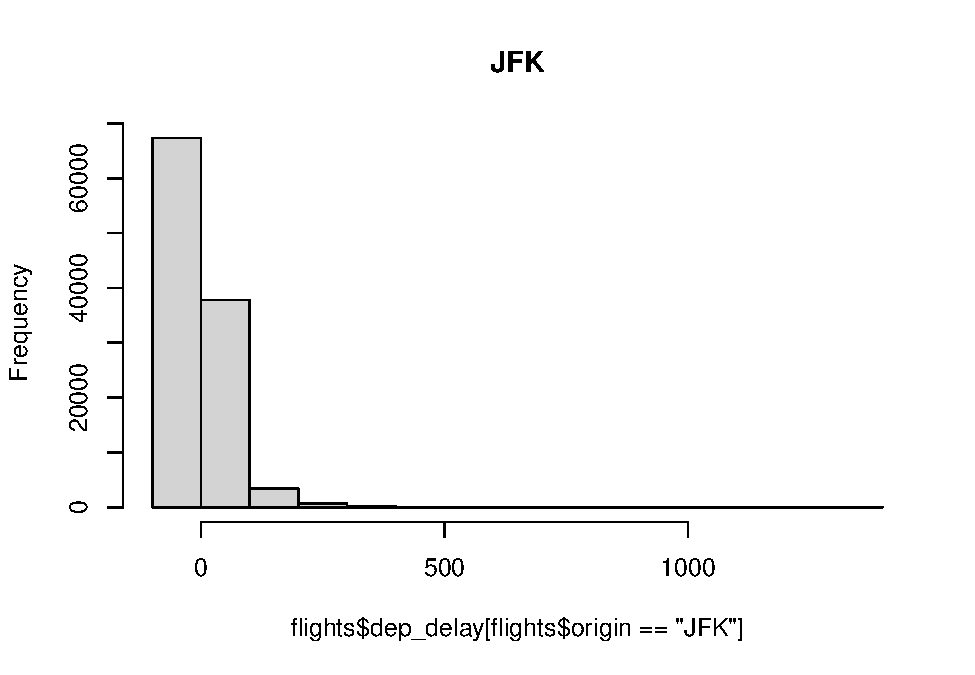
\includegraphics{AprendendoR_files/figure-latex/unnamed-chunk-27-1.pdf}

\begin{Shaded}
\begin{Highlighting}[]
\FunctionTok{hist}\NormalTok{(flights}\SpecialCharTok{$}\NormalTok{dep\_delay[flights}\SpecialCharTok{$}\NormalTok{origin }\SpecialCharTok{==} \StringTok{"LGA"}\NormalTok{], }\AttributeTok{main=}\StringTok{"LGA"}\NormalTok{)}
\end{Highlighting}
\end{Shaded}

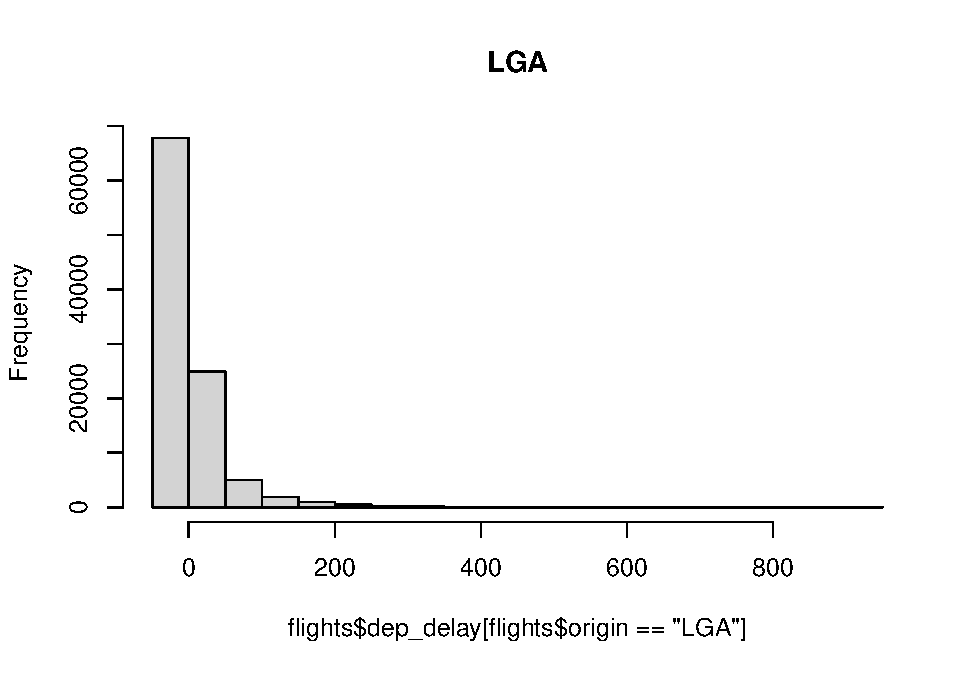
\includegraphics{AprendendoR_files/figure-latex/unnamed-chunk-27-2.pdf}

\begin{Shaded}
\begin{Highlighting}[]
\FunctionTok{hist}\NormalTok{(flights}\SpecialCharTok{$}\NormalTok{dep\_delay[flights}\SpecialCharTok{$}\NormalTok{origin }\SpecialCharTok{==} \StringTok{"EWR"}\NormalTok{], }\AttributeTok{main=}\StringTok{"EWR"}\NormalTok{)}
\end{Highlighting}
\end{Shaded}

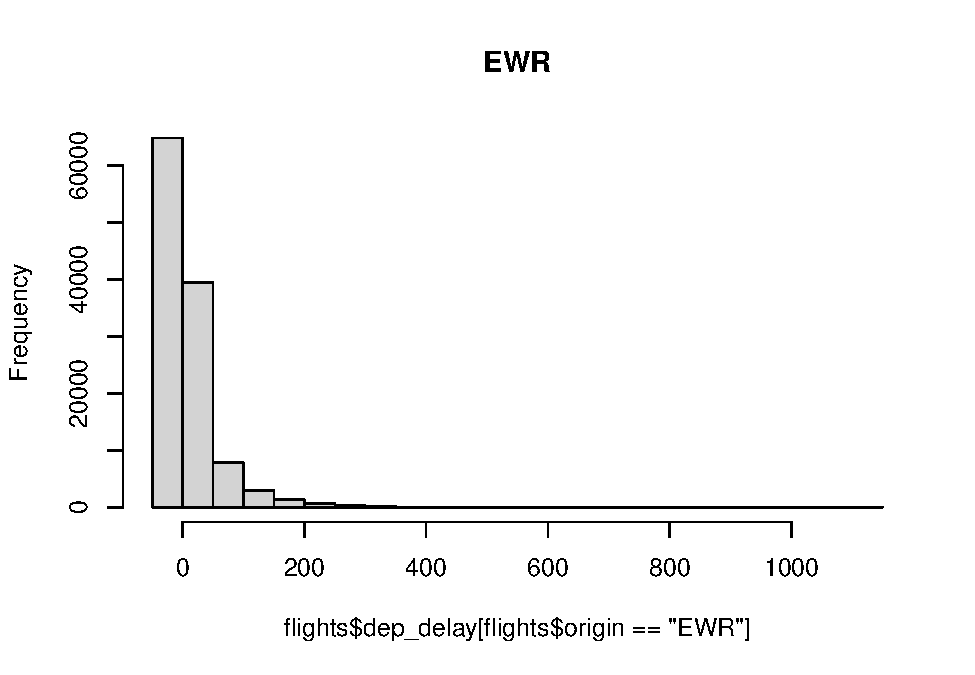
\includegraphics{AprendendoR_files/figure-latex/unnamed-chunk-27-3.pdf}

Os três gráficos podem ser exibidos de uma única vez se usarmos a opção \texttt{mfrow}, que permite definir o número de linhas e colunas do grid para plotar os gráficos.

\begin{Shaded}
\begin{Highlighting}[]
\FunctionTok{par}\NormalTok{(}\AttributeTok{mfrow=}\FunctionTok{c}\NormalTok{(}\DecValTok{1}\NormalTok{,}\DecValTok{3}\NormalTok{))}

\FunctionTok{hist}\NormalTok{(flights}\SpecialCharTok{$}\NormalTok{dep\_delay[flights}\SpecialCharTok{$}\NormalTok{origin }\SpecialCharTok{==} \StringTok{"JFK"}\NormalTok{], }\AttributeTok{main=}\StringTok{"JFK"}\NormalTok{)}

\FunctionTok{hist}\NormalTok{(flights}\SpecialCharTok{$}\NormalTok{dep\_delay[flights}\SpecialCharTok{$}\NormalTok{origin }\SpecialCharTok{==} \StringTok{"LGA"}\NormalTok{], }\AttributeTok{main=}\StringTok{"LGA"}\NormalTok{)}

\FunctionTok{hist}\NormalTok{(flights}\SpecialCharTok{$}\NormalTok{dep\_delay[flights}\SpecialCharTok{$}\NormalTok{origin }\SpecialCharTok{==} \StringTok{"EWR"}\NormalTok{], }\AttributeTok{main=}\StringTok{"EWR"}\NormalTok{)}
\end{Highlighting}
\end{Shaded}

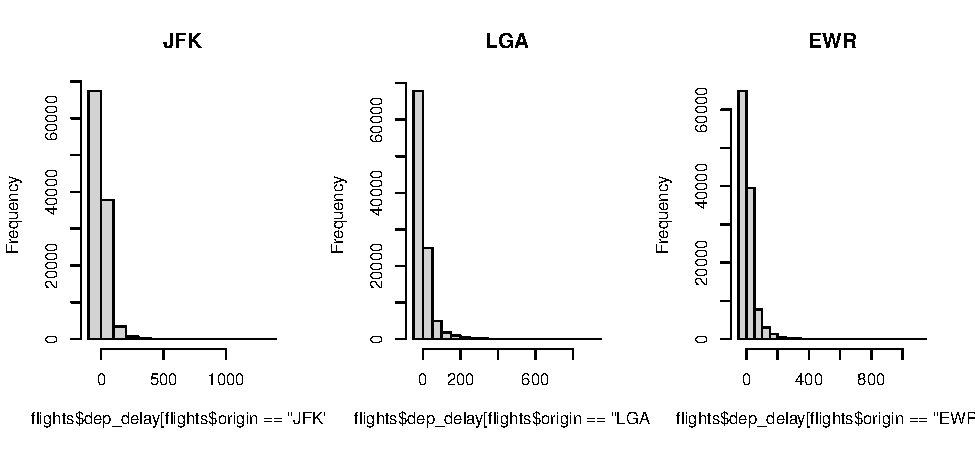
\includegraphics[width=1\linewidth]{AprendendoR_files/figure-latex/unnamed-chunk-28-1}

\section{Lista de exercicios}\label{lista-de-exercicios-1}

\begin{enumerate}
\def\labelenumi{\arabic{enumi}.}
\item
  Importe no \texttt{R} a planilha de dados correspondente ao seu projeto aplicado.
\item
  Verifique se alguma coluna deve ser transformada para um tipo de dados mais adequado.
\item
  Obtenha estatísticas descritivas dos dados.
\end{enumerate}

\chapter{\texorpdfstring{O pacote \texttt{tidyverse}}{O pacote tidyverse}}\label{o-pacote-tidyverse}

\begin{quote}
Este capítulo foi baseado no livro \href{https://r4ds.had.co.nz/}{R for Data Science}, que atualmente está sendo traduzido para o português brasileiro através de um grupo de pessoas voluntárias (\href{https://github.com/orgs/cienciadedatos/projects/2}{mais detalhes aqui}).
\end{quote}

\texttt{tidyverse} é uma coleção de bibliotecas criadas para o universo de data science.
Todos os pacotes `tidyverse' possuem a mesma gramática, estrutura de dados e filosofia:

Veja todos os pacotes disponíveis em: \url{https://www.tidyverse.org/}

Vamos instalar o pacote \texttt{tidyverse}:

\begin{Shaded}
\begin{Highlighting}[]
\FunctionTok{install.packages}\NormalTok{(}\StringTok{"tidyverse"}\NormalTok{)}
\end{Highlighting}
\end{Shaded}

E carregar a biblioteca:

\begin{Shaded}
\begin{Highlighting}[]
\FunctionTok{library}\NormalTok{(tidyverse)}
\end{Highlighting}
\end{Shaded}

\begin{verbatim}
## -- Attaching packages --------------------------------------- tidyverse 1.3.2 --
## v ggplot2 3.4.2      v purrr   0.3.5 
## v tibble  3.2.1      v dplyr   1.0.10
## v tidyr   1.2.1      v stringr 1.4.1 
## v readr   2.1.3      v forcats 0.5.2
\end{verbatim}

\begin{verbatim}
## Warning: package 'ggplot2' was built under R version 4.2.3
\end{verbatim}

\begin{verbatim}
## Warning: package 'tibble' was built under R version 4.2.3
\end{verbatim}

\begin{verbatim}
## -- Conflicts ------------------------------------------ tidyverse_conflicts() --
## x lubridate::as.difftime() masks base::as.difftime()
## x lubridate::date()        masks base::date()
## x dplyr::filter()          masks stats::filter()
## x lubridate::intersect()   masks base::intersect()
## x dplyr::lag()             masks stats::lag()
## x lubridate::setdiff()     masks base::setdiff()
## x lubridate::union()       masks base::union()
\end{verbatim}

\section{\texorpdfstring{O operador pipe ( \%\textgreater\% ) da library \texttt{magrittr}}{O operador pipe ( \%\textgreater\% ) da library magrittr}}\label{o-operador-pipe-da-library-magrittr}

Atalho no teclado: \texttt{Ctrl\ +\ Shift\ +\ M}

Passa o objeto do lado esquerdo como primeiro argumento (ou
.argumento) da função do lado direito:

\begin{itemize}
\item
  \textbf{x} \texttt{\%\textgreater{}\%} f(y) é equivalente a f(\textbf{x},y)
\item
  \textbf{y} \texttt{\%\textgreater{}\%} f(x,\texttt{.},z) é equivalente a f(x,\textbf{y},z)
\end{itemize}

Na prática, vamos supor que queremos somar todos os elementos do \texttt{vetor} e em seguida tirar a raiz quadrada desta soma:

\begin{Shaded}
\begin{Highlighting}[]
\NormalTok{vetor }\OtherTok{\textless{}{-}} \FunctionTok{c}\NormalTok{(}\DecValTok{20}\NormalTok{,}\DecValTok{40}\NormalTok{,}\DecValTok{60}\NormalTok{,}\DecValTok{80}\NormalTok{,}\DecValTok{200}\NormalTok{)}

\CommentTok{\#raiz da soma}
\FunctionTok{sqrt}\NormalTok{(}\FunctionTok{sum}\NormalTok{(vetor))}
\end{Highlighting}
\end{Shaded}

\begin{verbatim}
## [1] 20
\end{verbatim}

Usando o pipe:

\begin{Shaded}
\begin{Highlighting}[]
\NormalTok{vetor }\SpecialCharTok{\%\textgreater{}\%} \FunctionTok{sum}\NormalTok{() }\SpecialCharTok{\%\textgreater{}\%} \FunctionTok{sqrt}\NormalTok{()}
\end{Highlighting}
\end{Shaded}

\begin{verbatim}
## [1] 20
\end{verbatim}

\section{\texorpdfstring{Transformação de Dados com \texttt{dplyr}}{Transformação de Dados com dplyr}}\label{transformauxe7uxe3o-de-dados-com-dplyr}

As cinco principais funções do \texttt{dplyr} são:

\begin{itemize}
\tightlist
\item
  \texttt{filter()}
  \vspace{3mm}
\item
  \texttt{arrange()}
  \vspace{3mm}
\item
  \texttt{select()}
  \vspace{3mm}
\item
  \texttt{mutate()}
  \vspace{3mm}
\item
  \texttt{summarize()}
\end{itemize}

Todos os verbos funcionam de maneira similar:

\begin{enumerate}
\def\labelenumi{\arabic{enumi}.}
\tightlist
\item
  O primeiro argumento é um data frame
  \vspace{2mm}
\item
  Os próximos argumentos descrevem o que fazer com o data frame
  \vspace{2mm}
\item
  O resultado é um novo data frame
\end{enumerate}

\section{\texorpdfstring{Filtrando linhas com \texttt{filter()}}{Filtrando linhas com filter()}}\label{filtrando-linhas-com-filter}

Vamos voltar a utilizar a base de dados flights:

\begin{Shaded}
\begin{Highlighting}[]
\NormalTok{flights }\OtherTok{\textless{}{-}} \FunctionTok{read.csv}\NormalTok{(}\StringTok{"flights.csv"}\NormalTok{)}
\end{Highlighting}
\end{Shaded}

Sem pipe:

\begin{Shaded}
\begin{Highlighting}[]
\FunctionTok{filter}\NormalTok{(flights, month }\SpecialCharTok{==} \DecValTok{1}\NormalTok{, day }\SpecialCharTok{==} \DecValTok{1}\NormalTok{)}
\end{Highlighting}
\end{Shaded}

\begin{verbatim}
## # A tibble: 842 x 19
##     year month   day dep_time sched_dep_time dep_delay arr_time sched_arr_time
##    <int> <int> <int>    <int>          <int>     <dbl>    <int>          <int>
##  1  2013     1     1      517            515         2      830            819
##  2  2013     1     1      533            529         4      850            830
##  3  2013     1     1      542            540         2      923            850
##  4  2013     1     1      544            545        -1     1004           1022
##  5  2013     1     1      554            600        -6      812            837
##  6  2013     1     1      554            558        -4      740            728
##  7  2013     1     1      555            600        -5      913            854
##  8  2013     1     1      557            600        -3      709            723
##  9  2013     1     1      557            600        -3      838            846
## 10  2013     1     1      558            600        -2      753            745
## # i 832 more rows
## # i 11 more variables: arr_delay <dbl>, carrier <chr>, flight <int>,
## #   tailnum <chr>, origin <chr>, dest <chr>, air_time <dbl>, distance <dbl>,
## #   hour <dbl>, minute <dbl>, time_hour <dttm>
\end{verbatim}

Com pipe:

\begin{Shaded}
\begin{Highlighting}[]
\NormalTok{flights }\SpecialCharTok{\%\textgreater{}\%} \FunctionTok{filter}\NormalTok{(month }\SpecialCharTok{==} \DecValTok{1}\NormalTok{, day }\SpecialCharTok{==} \DecValTok{1}\NormalTok{)}
\end{Highlighting}
\end{Shaded}

\begin{verbatim}
## # A tibble: 842 x 19
##     year month   day dep_time sched_dep_time dep_delay arr_time sched_arr_time
##    <int> <int> <int>    <int>          <int>     <dbl>    <int>          <int>
##  1  2013     1     1      517            515         2      830            819
##  2  2013     1     1      533            529         4      850            830
##  3  2013     1     1      542            540         2      923            850
##  4  2013     1     1      544            545        -1     1004           1022
##  5  2013     1     1      554            600        -6      812            837
##  6  2013     1     1      554            558        -4      740            728
##  7  2013     1     1      555            600        -5      913            854
##  8  2013     1     1      557            600        -3      709            723
##  9  2013     1     1      557            600        -3      838            846
## 10  2013     1     1      558            600        -2      753            745
## # i 832 more rows
## # i 11 more variables: arr_delay <dbl>, carrier <chr>, flight <int>,
## #   tailnum <chr>, origin <chr>, dest <chr>, air_time <dbl>, distance <dbl>,
## #   hour <dbl>, minute <dbl>, time_hour <dttm>
\end{verbatim}

Atrubuindo e imprimindo:

\begin{Shaded}
\begin{Highlighting}[]
\CommentTok{\# Para atribuir e imprimir de uma só vez, coloque}
\CommentTok{\# parênteses em volta da atribuição (os dois espaços}
\CommentTok{\# depois dos parênteses abaixo não são necessários).}

\NormalTok{(  jan1 }\OtherTok{\textless{}{-}}\NormalTok{ flights }\SpecialCharTok{\%\textgreater{}\%} \FunctionTok{filter}\NormalTok{(month }\SpecialCharTok{==} \DecValTok{1}\NormalTok{, day }\SpecialCharTok{==} \DecValTok{1}\NormalTok{)  )}
\end{Highlighting}
\end{Shaded}

\begin{verbatim}
## # A tibble: 842 x 19
##     year month   day dep_time sched_dep_time dep_delay arr_time sched_arr_time
##    <int> <int> <int>    <int>          <int>     <dbl>    <int>          <int>
##  1  2013     1     1      517            515         2      830            819
##  2  2013     1     1      533            529         4      850            830
##  3  2013     1     1      542            540         2      923            850
##  4  2013     1     1      544            545        -1     1004           1022
##  5  2013     1     1      554            600        -6      812            837
##  6  2013     1     1      554            558        -4      740            728
##  7  2013     1     1      555            600        -5      913            854
##  8  2013     1     1      557            600        -3      709            723
##  9  2013     1     1      557            600        -3      838            846
## 10  2013     1     1      558            600        -2      753            745
## # i 832 more rows
## # i 11 more variables: arr_delay <dbl>, carrier <chr>, flight <int>,
## #   tailnum <chr>, origin <chr>, dest <chr>, air_time <dbl>, distance <dbl>,
## #   hour <dbl>, minute <dbl>, time_hour <dttm>
\end{verbatim}

\newpage

Podemos utilizar os operadores lógicos aprendidos nas primeiras aulas para filtrar aqui também.

Por exemplo, vamos filtar somente as observações que \textbf{não} são \texttt{NA} na coluna \texttt{arr\_delay}:

\begin{Shaded}
\begin{Highlighting}[]
\NormalTok{flights }\SpecialCharTok{\%\textgreater{}\%} \FunctionTok{filter}\NormalTok{(}\SpecialCharTok{!}\FunctionTok{is.na}\NormalTok{(arr\_delay))}
\end{Highlighting}
\end{Shaded}

\begin{verbatim}
## # A tibble: 327,346 x 19
##     year month   day dep_time sched_dep_time dep_delay arr_time sched_arr_time
##    <int> <int> <int>    <int>          <int>     <dbl>    <int>          <int>
##  1  2013     1     1      517            515         2      830            819
##  2  2013     1     1      533            529         4      850            830
##  3  2013     1     1      542            540         2      923            850
##  4  2013     1     1      544            545        -1     1004           1022
##  5  2013     1     1      554            600        -6      812            837
##  6  2013     1     1      554            558        -4      740            728
##  7  2013     1     1      555            600        -5      913            854
##  8  2013     1     1      557            600        -3      709            723
##  9  2013     1     1      557            600        -3      838            846
## 10  2013     1     1      558            600        -2      753            745
## # i 327,336 more rows
## # i 11 more variables: arr_delay <dbl>, carrier <chr>, flight <int>,
## #   tailnum <chr>, origin <chr>, dest <chr>, air_time <dbl>, distance <dbl>,
## #   hour <dbl>, minute <dbl>, time_hour <dttm>
\end{verbatim}

Origem = Kennedy ou Newark, Destino = Los Angeles:

\begin{Shaded}
\begin{Highlighting}[]
\NormalTok{flights }\SpecialCharTok{\%\textgreater{}\%} \FunctionTok{filter}\NormalTok{(origin }\SpecialCharTok{\%in\%} \FunctionTok{c}\NormalTok{(}\StringTok{"JFK"}\NormalTok{, }\StringTok{"EWR"}\NormalTok{), dest }\SpecialCharTok{==} \StringTok{"LAX"}\NormalTok{)}
\end{Highlighting}
\end{Shaded}

\begin{verbatim}
## # A tibble: 16,174 x 19
##     year month   day dep_time sched_dep_time dep_delay arr_time sched_arr_time
##    <int> <int> <int>    <int>          <int>     <dbl>    <int>          <int>
##  1  2013     1     1      558            600        -2      924            917
##  2  2013     1     1      628            630        -2     1016            947
##  3  2013     1     1      658            700        -2     1027           1025
##  4  2013     1     1      702            700         2     1058           1014
##  5  2013     1     1      743            730        13     1107           1100
##  6  2013     1     1      828            823         5     1150           1143
##  7  2013     1     1      829            830        -1     1152           1200
##  8  2013     1     1      856            900        -4     1226           1220
##  9  2013     1     1      859            900        -1     1223           1225
## 10  2013     1     1      921            900        21     1237           1227
## # i 16,164 more rows
## # i 11 more variables: arr_delay <dbl>, carrier <chr>, flight <int>,
## #   tailnum <chr>, origin <chr>, dest <chr>, air_time <dbl>, distance <dbl>,
## #   hour <dbl>, minute <dbl>, time_hour <dttm>
\end{verbatim}

\newpage

\section{\texorpdfstring{Arranjando linhas com \texttt{arrange()}}{Arranjando linhas com arrange()}}\label{arranjando-linhas-com-arrange}

Organizando os dados segundo a ordem crescente da coluna \texttt{dep\_delay}:

\begin{Shaded}
\begin{Highlighting}[]
\NormalTok{flights }\SpecialCharTok{\%\textgreater{}\%} \FunctionTok{arrange}\NormalTok{(dep\_delay)}
\end{Highlighting}
\end{Shaded}

\begin{verbatim}
## # A tibble: 336,776 x 19
##     year month   day dep_time sched_dep_time dep_delay arr_time sched_arr_time
##    <int> <int> <int>    <int>          <int>     <dbl>    <int>          <int>
##  1  2013    12     7     2040           2123       -43       40           2352
##  2  2013     2     3     2022           2055       -33     2240           2338
##  3  2013    11    10     1408           1440       -32     1549           1559
##  4  2013     1    11     1900           1930       -30     2233           2243
##  5  2013     1    29     1703           1730       -27     1947           1957
##  6  2013     8     9      729            755       -26     1002            955
##  7  2013    10    23     1907           1932       -25     2143           2143
##  8  2013     3    30     2030           2055       -25     2213           2250
##  9  2013     3     2     1431           1455       -24     1601           1631
## 10  2013     5     5      934            958       -24     1225           1309
## # i 336,766 more rows
## # i 11 more variables: arr_delay <dbl>, carrier <chr>, flight <int>,
## #   tailnum <chr>, origin <chr>, dest <chr>, air_time <dbl>, distance <dbl>,
## #   hour <dbl>, minute <dbl>, time_hour <dttm>
\end{verbatim}

Agora usando a ordem decrescente:

\begin{Shaded}
\begin{Highlighting}[]
\NormalTok{flights }\SpecialCharTok{\%\textgreater{}\%} \FunctionTok{arrange}\NormalTok{(}\FunctionTok{desc}\NormalTok{(dep\_delay))}
\end{Highlighting}
\end{Shaded}

\begin{verbatim}
## # A tibble: 336,776 x 19
##     year month   day dep_time sched_dep_time dep_delay arr_time sched_arr_time
##    <int> <int> <int>    <int>          <int>     <dbl>    <int>          <int>
##  1  2013     1     9      641            900      1301     1242           1530
##  2  2013     6    15     1432           1935      1137     1607           2120
##  3  2013     1    10     1121           1635      1126     1239           1810
##  4  2013     9    20     1139           1845      1014     1457           2210
##  5  2013     7    22      845           1600      1005     1044           1815
##  6  2013     4    10     1100           1900       960     1342           2211
##  7  2013     3    17     2321            810       911      135           1020
##  8  2013     6    27      959           1900       899     1236           2226
##  9  2013     7    22     2257            759       898      121           1026
## 10  2013    12     5      756           1700       896     1058           2020
## # i 336,766 more rows
## # i 11 more variables: arr_delay <dbl>, carrier <chr>, flight <int>,
## #   tailnum <chr>, origin <chr>, dest <chr>, air_time <dbl>, distance <dbl>,
## #   hour <dbl>, minute <dbl>, time_hour <dttm>
\end{verbatim}

Se você fornecer mais de uma coluna, as demais colunas serão usadas sucessivamente para decidir os empates:

\begin{Shaded}
\begin{Highlighting}[]
\NormalTok{flights }\SpecialCharTok{\%\textgreater{}\%} \FunctionTok{arrange}\NormalTok{(}\FunctionTok{desc}\NormalTok{(month), day)}
\end{Highlighting}
\end{Shaded}

\begin{verbatim}
## # A tibble: 336,776 x 19
##     year month   day dep_time sched_dep_time dep_delay arr_time sched_arr_time
##    <int> <int> <int>    <int>          <int>     <dbl>    <int>          <int>
##  1  2013    12     1       13           2359        14      446            445
##  2  2013    12     1       17           2359        18      443            437
##  3  2013    12     1      453            500        -7      636            651
##  4  2013    12     1      520            515         5      749            808
##  5  2013    12     1      536            540        -4      845            850
##  6  2013    12     1      540            550       -10     1005           1027
##  7  2013    12     1      541            545        -4      734            755
##  8  2013    12     1      546            545         1      826            835
##  9  2013    12     1      549            600       -11      648            659
## 10  2013    12     1      550            600       -10      825            854
## # i 336,766 more rows
## # i 11 more variables: arr_delay <dbl>, carrier <chr>, flight <int>,
## #   tailnum <chr>, origin <chr>, dest <chr>, air_time <dbl>, distance <dbl>,
## #   hour <dbl>, minute <dbl>, time_hour <dttm>
\end{verbatim}

\section{Selecionando colunas com select()}\label{selecionando-colunas-com-select}

Vamos supor que eu só queira utilizar colunas específicas da minha base: \texttt{carrier}, \texttt{year}, \texttt{month} e \texttt{day}

\begin{Shaded}
\begin{Highlighting}[]
\NormalTok{flights }\SpecialCharTok{\%\textgreater{}\%} \FunctionTok{select}\NormalTok{(carrier, year, month, day)}
\end{Highlighting}
\end{Shaded}

\begin{verbatim}
## # A tibble: 336,776 x 4
##    carrier  year month   day
##    <chr>   <int> <int> <int>
##  1 UA       2013     1     1
##  2 UA       2013     1     1
##  3 AA       2013     1     1
##  4 B6       2013     1     1
##  5 DL       2013     1     1
##  6 UA       2013     1     1
##  7 B6       2013     1     1
##  8 EV       2013     1     1
##  9 B6       2013     1     1
## 10 AA       2013     1     1
## # i 336,766 more rows
\end{verbatim}

Selecionando todas as colunas, MENOS a coluna \texttt{year}:

\begin{Shaded}
\begin{Highlighting}[]
\NormalTok{flights }\SpecialCharTok{\%\textgreater{}\%} \FunctionTok{select}\NormalTok{(}\SpecialCharTok{{-}}\NormalTok{year)}
\end{Highlighting}
\end{Shaded}

\begin{verbatim}
## # A tibble: 336,776 x 18
##    month   day dep_time sched_dep_time dep_delay arr_time sched_arr_time
##    <int> <int>    <int>          <int>     <dbl>    <int>          <int>
##  1     1     1      517            515         2      830            819
##  2     1     1      533            529         4      850            830
##  3     1     1      542            540         2      923            850
##  4     1     1      544            545        -1     1004           1022
##  5     1     1      554            600        -6      812            837
##  6     1     1      554            558        -4      740            728
##  7     1     1      555            600        -5      913            854
##  8     1     1      557            600        -3      709            723
##  9     1     1      557            600        -3      838            846
## 10     1     1      558            600        -2      753            745
## # i 336,766 more rows
## # i 11 more variables: arr_delay <dbl>, carrier <chr>, flight <int>,
## #   tailnum <chr>, origin <chr>, dest <chr>, air_time <dbl>, distance <dbl>,
## #   hour <dbl>, minute <dbl>, time_hour <dttm>
\end{verbatim}

\texttt{everything()} é útil para mover as colunas de lugar:

\begin{Shaded}
\begin{Highlighting}[]
\NormalTok{flights }\SpecialCharTok{\%\textgreater{}\%} \FunctionTok{select}\NormalTok{(carrier, origin, }\FunctionTok{everything}\NormalTok{())}
\end{Highlighting}
\end{Shaded}

\begin{verbatim}
## # A tibble: 336,776 x 19
##    carrier origin  year month   day dep_time sched_dep_time dep_delay arr_time
##    <chr>   <chr>  <int> <int> <int>    <int>          <int>     <dbl>    <int>
##  1 UA      EWR     2013     1     1      517            515         2      830
##  2 UA      LGA     2013     1     1      533            529         4      850
##  3 AA      JFK     2013     1     1      542            540         2      923
##  4 B6      JFK     2013     1     1      544            545        -1     1004
##  5 DL      LGA     2013     1     1      554            600        -6      812
##  6 UA      EWR     2013     1     1      554            558        -4      740
##  7 B6      EWR     2013     1     1      555            600        -5      913
##  8 EV      LGA     2013     1     1      557            600        -3      709
##  9 B6      JFK     2013     1     1      557            600        -3      838
## 10 AA      LGA     2013     1     1      558            600        -2      753
## # i 336,766 more rows
## # i 10 more variables: sched_arr_time <int>, arr_delay <dbl>, flight <int>,
## #   tailnum <chr>, dest <chr>, air_time <dbl>, distance <dbl>, hour <dbl>,
## #   minute <dbl>, time_hour <dttm>
\end{verbatim}

Também podemos renomear uma coluna dentro do select:

\begin{Shaded}
\begin{Highlighting}[]
\CommentTok{\#renomeando a coluna year para "ano":}

\NormalTok{flights }\SpecialCharTok{\%\textgreater{}\%} \FunctionTok{select}\NormalTok{(}\StringTok{"ano"} \OtherTok{=}\NormalTok{ year, month, day)}
\end{Highlighting}
\end{Shaded}

\begin{verbatim}
## # A tibble: 336,776 x 3
##      ano month   day
##    <int> <int> <int>
##  1  2013     1     1
##  2  2013     1     1
##  3  2013     1     1
##  4  2013     1     1
##  5  2013     1     1
##  6  2013     1     1
##  7  2013     1     1
##  8  2013     1     1
##  9  2013     1     1
## 10  2013     1     1
## # i 336,766 more rows
\end{verbatim}

Combinando \texttt{filter()}, \texttt{select()} e \texttt{arrange()}:

Suponha que nosso objetivo seja verificar qual a companhia aérea que mais atrasa nos vôos entre JFK e LAX:

\begin{Shaded}
\begin{Highlighting}[]
\NormalTok{flights }\SpecialCharTok{\%\textgreater{}\%}
    \FunctionTok{filter}\NormalTok{(origin }\SpecialCharTok{==} \StringTok{"JFK"}\NormalTok{, dest }\SpecialCharTok{==} \StringTok{"LAX"}\NormalTok{) }\SpecialCharTok{\%\textgreater{}\%}
    \FunctionTok{select}\NormalTok{(carrier, dep\_delay) }\SpecialCharTok{\%\textgreater{}\%}
    \FunctionTok{arrange}\NormalTok{(}\FunctionTok{desc}\NormalTok{(dep\_delay))}
\end{Highlighting}
\end{Shaded}

\begin{verbatim}
## # A tibble: 11,262 x 2
##    carrier dep_delay
##    <chr>       <dbl>
##  1 DL            800
##  2 VX            634
##  3 VX            434
##  4 VX            413
##  5 VX            392
##  6 UA            364
##  7 AA            345
##  8 AA            334
##  9 VX            322
## 10 AA            321
## # i 11,252 more rows
\end{verbatim}

\section{\texorpdfstring{Criando variáveis (colunas) com \texttt{mutate()}}{Criando variáveis (colunas) com mutate()}}\label{criando-variuxe1veis-colunas-com-mutate}

Queremos criar uma variável que mostre a velocidade de cada voo:

\begin{Shaded}
\begin{Highlighting}[]
\NormalTok{flights }\SpecialCharTok{\%\textgreater{}\%}
    \FunctionTok{select}\NormalTok{(year}\SpecialCharTok{:}\NormalTok{day, flight,  distance, air\_time) }\SpecialCharTok{\%\textgreater{}\%}
    \FunctionTok{mutate}\NormalTok{(}\AttributeTok{speed =}\NormalTok{ distance }\SpecialCharTok{/}\NormalTok{ (air\_time }\SpecialCharTok{/} \DecValTok{60}\NormalTok{))}
\end{Highlighting}
\end{Shaded}

\begin{verbatim}
## # A tibble: 336,776 x 7
##     year month   day flight distance air_time speed
##    <int> <int> <int>  <int>    <dbl>    <dbl> <dbl>
##  1  2013     1     1   1545     1400      227  370.
##  2  2013     1     1   1714     1416      227  374.
##  3  2013     1     1   1141     1089      160  408.
##  4  2013     1     1    725     1576      183  517.
##  5  2013     1     1    461      762      116  394.
##  6  2013     1     1   1696      719      150  288.
##  7  2013     1     1    507     1065      158  404.
##  8  2013     1     1   5708      229       53  259.
##  9  2013     1     1     79      944      140  405.
## 10  2013     1     1    301      733      138  319.
## # i 336,766 more rows
\end{verbatim}

Note que você também pode se referir às variáveis que criou:

\begin{Shaded}
\begin{Highlighting}[]
\NormalTok{flights }\SpecialCharTok{\%\textgreater{}\%}
    \FunctionTok{select}\NormalTok{(year}\SpecialCharTok{:}\NormalTok{day, flight,  distance, air\_time) }\SpecialCharTok{\%\textgreater{}\%}
    \FunctionTok{mutate}\NormalTok{(}\AttributeTok{hours =}\NormalTok{ air\_time }\SpecialCharTok{/} \DecValTok{60}\NormalTok{,}
           \AttributeTok{speed =}\NormalTok{ distance }\SpecialCharTok{/}\NormalTok{ hours)}
\end{Highlighting}
\end{Shaded}

\begin{verbatim}
## # A tibble: 336,776 x 8
##     year month   day flight distance air_time hours speed
##    <int> <int> <int>  <int>    <dbl>    <dbl> <dbl> <dbl>
##  1  2013     1     1   1545     1400      227 3.78   370.
##  2  2013     1     1   1714     1416      227 3.78   374.
##  3  2013     1     1   1141     1089      160 2.67   408.
##  4  2013     1     1    725     1576      183 3.05   517.
##  5  2013     1     1    461      762      116 1.93   394.
##  6  2013     1     1   1696      719      150 2.5    288.
##  7  2013     1     1    507     1065      158 2.63   404.
##  8  2013     1     1   5708      229       53 0.883  259.
##  9  2013     1     1     79      944      140 2.33   405.
## 10  2013     1     1    301      733      138 2.3    319.
## # i 336,766 more rows
\end{verbatim}

\section{\texorpdfstring{\texttt{summarise()} colapsa a tabela toda em apenas uma linha}{summarise() colapsa a tabela toda em apenas uma linha}}\label{summarise-colapsa-a-tabela-toda-em-apenas-uma-linha}

Vamos calcular o atraso médio de decolagem e a quantidade total de voos:

\begin{Shaded}
\begin{Highlighting}[]
\NormalTok{flights }\SpecialCharTok{\%\textgreater{}\%}
    \FunctionTok{filter}\NormalTok{(}\SpecialCharTok{!}\FunctionTok{is.na}\NormalTok{(dep\_delay)) }\SpecialCharTok{\%\textgreater{}\%}
    \FunctionTok{summarise}\NormalTok{(}\AttributeTok{mean\_delay =} \FunctionTok{mean}\NormalTok{(dep\_delay), }\AttributeTok{number\_of\_flights =} \FunctionTok{n}\NormalTok{())}
\end{Highlighting}
\end{Shaded}

\begin{verbatim}
## # A tibble: 1 x 2
##   mean_delay number_of_flights
##        <dbl>             <int>
## 1       12.6            328521
\end{verbatim}

\section{\texorpdfstring{\texttt{group\_by()} muda a ``unidade de análise'' de toda a tabela para os grupos definidos}{group\_by() muda a ``unidade de análise'' de toda a tabela para os grupos definidos}}\label{group_by-muda-a-unidade-de-anuxe1lise-de-toda-a-tabela-para-os-grupos-definidos}

Vamos calcular o atraso médio de decolagem e a quantidade total de voos, mas agora analisando por companhia aérea:

\begin{Shaded}
\begin{Highlighting}[]
\NormalTok{flights }\SpecialCharTok{\%\textgreater{}\%}
    \FunctionTok{filter}\NormalTok{(}\SpecialCharTok{!}\FunctionTok{is.na}\NormalTok{(dep\_delay)) }\SpecialCharTok{\%\textgreater{}\%}
    \FunctionTok{group\_by}\NormalTok{(carrier) }\SpecialCharTok{\%\textgreater{}\%} 
    \FunctionTok{summarise}\NormalTok{(}\AttributeTok{mean\_delay =} \FunctionTok{mean}\NormalTok{(dep\_delay), }\AttributeTok{number\_of\_flights =} \FunctionTok{n}\NormalTok{())}
\end{Highlighting}
\end{Shaded}

\begin{verbatim}
## # A tibble: 16 x 3
##    carrier mean_delay number_of_flights
##    <chr>        <dbl>             <int>
##  1 9E           16.7              17416
##  2 AA            8.59             32093
##  3 AS            5.80               712
##  4 B6           13.0              54169
##  5 DL            9.26             47761
##  6 EV           20.0              51356
##  7 F9           20.2                682
##  8 FL           18.7               3187
##  9 HA            4.90               342
## 10 MQ           10.6              25163
## 11 OO           12.6                 29
## 12 UA           12.1              57979
## 13 US            3.78             19873
## 14 VX           12.9               5131
## 15 WN           17.7              12083
## 16 YV           19.0                545
\end{verbatim}

\subsection{DESAFIO:}\label{desafio}

Para cada destino, calcule: a (1) distância média dos voos e (2) o tempo de atraso médio na decolagem e (3) o número de voos na base e mostre tudo numa planilha só.

\chapter{\texorpdfstring{\texttt{ggplot}}{ggplot}}\label{ggplot}

Em breve!

\chapter*{References}\label{references}
\addcontentsline{toc}{chapter}{References}

\begin{itemize}
\item
  Cotton, R. (2013). Learning R: a step-by-step function guide to data analysis. '' O'Reilly Media, Inc.''.
\item
  Wickham, H., Çetinkaya-Rundel, M., \& Grolemund, G. (2023). \href{https://r4ds.had.co.nz/}{R for Data Science}. '' O'Reilly Media, Inc.''.
\end{itemize}

  \bibliography{book.bib,packages.bib}

\end{document}
